\documentclass{article}
\usepackage{mathtools}
\usepackage{amsmath}
\usepackage{amssymb}
\usepackage{amsthm}
\usepackage{systeme}
\usepackage{newtxtext}
\usepackage{newtxmath}
\usepackage{listings}
\usepackage{xcolor}
\usepackage{array}
\usepackage{makecell}
\usepackage{booktabs}% http://ctan.org/pkg/booktabs
\usepackage{float}
\usepackage{hyperref}
\usepackage{tikz}
\usepackage{multicol}
\usepackage[utf8]{inputenc}
\usepackage[english]{babel}

\usetikzlibrary{arrows.meta}

\restylefloat{table}
\newcommand{\tabitem}{~~\llap{\textbullet}~~}

\newtheorem{theorem}{Theorem}[section]
\newtheorem{corollary}{Corollary}[theorem]
\newtheorem{defn}{Definition}[section]
\newtheorem{lemma}[theorem]{Lemma}
\newtheorem{axiom}[theorem]{Axiom}

\newcommand{\curvedE}{\mathscr{e}}
\newcommand{\vVar}{\mathscr{v}_{var}}
\newcommand{\Var}{\mathbb{V}ar}
\newcommand{\vE}{\mathscr{v}}
\newcommand{\vBool}{\xi}
\newcommand{\Ts}{\mathcal{T}_s}
\newcommand{\signT}{\mathbb{T}}
\newcommand{\signF}{\mathbb{F}}
\newcommand{\BranchConjunction}{%
\begin{align*}
			\bigwedge_{i=1}^{I} \; C(a_i, b_i) \:\: & \wedge \:\: 
			\bigwedge_{k=1}^{K} \; \neg C(e_k, f_k) \:\: \wedge \:\: \\
			\bigwedge_{j=1}^{J} \; d_j \neq 0 \:\: & \wedge \:\:
			\bigwedge_{l=1}^{L} \; g_l = 0 \:\: \wedge \:\:\\
			\bigwedge_{p=1}^{P} \; m_p \le_\mu n_p \:\: &\wedge \:\:
			\bigwedge_{q=1}^{Q} \; u_q <_\mu v_q \:\:
\end{align*}%
}

\lstset { %
    language=C++,
    backgroundcolor=\color{black!5}, % set backgroundcolor
    basicstyle=\footnotesize,% basic font setting
}

\title{Satisfiability of Quantitative Contact Logics}
\date{2019-9-28}
\author{Martin Stoev}

\begin{document}
	\maketitle
 	\thispagestyle{empty}
	\newpage

	\tableofcontents
	\pagenumbering{arabic}

	\newpage
\begin{abstract}
	In this paper an algorithm is defined for proving the satisfiability of formulas defined in the space of the quantitative contact logics.When a formula is not satisfiable then a model to satisfy the formula does not exist. In case the formula is satisfiable the algorithm constructs a model which satisfies the formula.
\end{abstract}
	\section{Introduction}
	The modal logics are in a constant exploration and extended by the today's researchers. The contact modal logics is one such topic with increasing interests. This paper works its way to an algorithm which for a given contact modal logics formula constructs a model which satisfies the formula. If such a model does not exist then the algorithm proves that the formula is not satisfiable. 

The model construction process begins with a formal prove procedure to decompose the formula to a simpler state. For this the tableau method is used. The tableau method branches the formula in many paths where each path is possible to derive a valid model for the formula. The procedure of model building is done for each path, until a model is successfully constructed. This procedure creates a modal points, the relations between them and the variables valuations in order to find a prove for a model satisfying the formula. 

As of today an algorithm which can solve this problem in a polynomial time is not possible. This is because the problem for constructing a satisfiable model for a quantitative contact formula is as hard as the Boolean satisfiability problem (SAT). That is why each optimization during the formula proving process is significantly reduces the algorithm execution time.

	\newpage
	\section{Tableaux Method}
	The tableau is a formal proof procedure which can be found in many variants and for different logics. In modal logics the tableau method is quite common and is mostly used for as a search procedure for models meeting certain conditions.
Formally, the tableau procedure is used as a refutation procedure; to prove that a formula X is satisfied, we begin the process with some syntactical assertion that the formula is not satisfiable. After that the assertion stating that the formula is not valid is broken down syntactically, in most cases breaking the formula into several cases. This decomposition of the initial formula is called tableau expansion stage and can be thought as a generalization of disjunctive normal form expansion. 

During the expansion stage of the tableau an impossible cases can be met, where the validity and invalidity of a formula are claimed to be true. These cases are said to be closed and if each case of the tableau is closed, then we say that the tableau is closed.

For our purposes, we will use a slightly different version of the method described above, namely with the help of the expansion stage we will try to find a model with certain properties in which the given formula will be satisfied.

		\subsection{Propositional logic tableau}
The tableau method for propositional logic is mostly defined based on the presentation of Raymond Smullyan. In its simplest form it is defined with syntactical assertion for the validity of the formula and definition of the expansion stage. To reach this goal, we need to improve our syntactical arsenal, to be able to assert the validity of a formula. In order to accomplish this, we shall introduce two signs. These signs when combined with a formula will assert whether the formula is true or false. Formally, the two signs are $\{ \signT, \signF \}$. Let $\varphi$ be a formula, then
\begin{itemize}
	\item $\signT \varphi$ - asserts the validity of the formula $\varphi$
	\item $\signF \varphi$ - asserts the invalidity of the formula $\varphi$
\end{itemize} 

The tableau of a formula $\varphi$ begins with $\signF \varphi$. The intuition behind it is that we start with an assertion that $\varphi$ is not valid in some model, and by decomposing the formula during the tableau process we seek for contradictions in the formals produced during the expansion stage. If such contradiction exists then the initial guess that the formula is not valid is not true; therefore the formula must be valid. On the other hand, if a contradiction does not exist then the formula is not valid. As mention above in our case the tableau will be used the other way around, namely for a given formula we will decompose it as much as possible (or until a contradiction is found) and then when there are no more possible ways to decompose the formula further we are going to seek a possible model which satisfies the formula $\varphi$. 

The expansion stage is a set of tableau steps, which decompose the initial formula into signed atomic formulas. A tableau expansion step applies one of the tableau rules to slightly simplify the given formula. There are two rules for each operation in the logic. In the case of propositional logic with the following operations $\{ \neg, \vee, \wedge, \rightarrow, \leftrightarrow \}$ there are ten rules. Each rule decomposes the formula in at most two formulas which depends on the arity of the operation. The expansion process forms branches. A branch contains signed formulas which have been asserted in the decomposition process.

A tableau rule which decomposes the formula in two formulas may require the assertion of only one of the produced formulas to be satisfied. In this case, we will say that the branch is split into two branches. However, in some terminologies this is noted as a new branch spawned from the original branch, or that two new branches are created. For the sake of simplicity, we will use the terminology of branch splitting. In a scenario where the branch is split, all asserted formulas in the branch are copied in the split branch together with the newly asserted formula from the tableau rule. The newly asserted formulas depend on the tableau rule.

	\subsection{Rules}
		\paragraph{Negation Rule}
The rules for negations are straightforward. When a negation operation is encountered, the sign of the captured formula changes.
		\newline
		\noindent\begin{minipage}{.5\linewidth}
		\begin{align*}
			\begin{array}{rl}
				& \signT(\neg \varphi), X \\
				      \cline{2-2}
				      & \signF(\varphi), X
			\end{array}
		\end{align*}
		\end{minipage}%
		\begin{minipage}{.5\linewidth}
		\begin{align*}
			\begin{array}{rl}
				& \signF(\neg \varphi), X \\
			      \cline{2-2}
			      & \signT(\varphi), X
			\end{array}
		\end{align*}
		\end{minipage}
		
		\paragraph{Conjunction Rule}
This is a binary operation, which means that the output of these rules is more complex than the negation rules.
The conjunction rule for a formula signed as valid decomposes the formula in two formulas and assert the validity of both of them.
On the other hand, the conjunction rule for a formula signed as invalid splits the branch into two branches and asserts the invalidity of the formulas in each branch, respectively.
		\newline
		\noindent\begin{minipage}{.5\linewidth}
		\begin{align*}
			\begin{array}{rl}
				& \signT(\varphi \: \wedge \: \psi), X \\
			      \cline{2-2}
			      & \signT\varphi, \signT\psi, X
			\end{array}
		\end{align*}
		\end{minipage}%
		\begin{minipage}{.5\linewidth}
		\begin{align*}
			\begin{array}{rl}
				& \:\:\: \signF(\varphi \: \wedge \: \psi), X \\
			      \cline{2-2}
			      & \signF\varphi, X \:\:\:\:\:\:\:\: \signF\psi, X
			\end{array}
		\end{align*}
		\end{minipage}

		\paragraph{Disjunction Rule}
This is a binary operation, which means that the output of these rules is more complex than the negation rules.
The disjunction rule for a formula signed as valid splits the branch into two branches and asserts the validity of the formulas in each branch, respectively.
On the other hand, the disjunction rule for a formula signed as invalid decomposes the formula in two formulas and assert the invalidity of both of them.
		\newline
		\noindent\begin{minipage}{.5\linewidth}
		\begin{align*}
			\begin{array}{rl}
				& \:\:\: \signT(\varphi \: \vee \: \psi), X \\
			      \cline{2-2}
			      & \signT\varphi, X \:\:\:\:\:\:\:\: \signT\psi, X
			\end{array}
		\end{align*}
		\end{minipage}%
		\begin{minipage}{.5\linewidth}
		\begin{align*}
			\begin{array}{rl}
				& \signF(\varphi \: \vee \: \psi), X \\
			      \cline{2-2}
			      & \signF\varphi, \signF\psi, X
			\end{array}
		\end{align*}
		\end{minipage}
		
		\paragraph{Implication}
The implication as well is a binary operation and depending on the asserting sign it decomposes the formula in two formulas or splits into two separate branches.
		\newline
		\noindent\begin{minipage}{.5\linewidth}
		\begin{align*}
			\begin{array}{rl}
				& \:\:\: \signT(\varphi \: \rightarrow \: \psi), X \\
			      \cline{2-2}
			      & \signF\varphi, X \:\:\:\:\:\:\:\: \signT\psi, X
			\end{array}
		\end{align*}
		\end{minipage}%
		\begin{minipage}{.5\linewidth}
		\begin{align*}
			\begin{array}{rl}
				& \signF(\varphi \: \rightarrow \: \psi), X \\
			      \cline{2-2}
			      & \signT\varphi, \signF\psi, X
			\end{array}
		\end{align*}
		\end{minipage}
		
		\paragraph{Equivalence}
Both of the equivalence rules split the branch into separate branches, the details can be observed in the following equations.
		\newline
		\noindent\begin{minipage}{.5\linewidth}
		\begin{align*}
			\begin{array}{rl}
				& \:\:\:\:\:\:\:\: \signT(\varphi \: \leftrightarrow \: \psi), X \\
			      \cline{2-2}
			      & \signT\varphi, \signT\psi, X \:\:\:\:\:\:\:\: \signF\varphi, \signF\psi, X
			\end{array}
		\end{align*}
		\end{minipage}%
		\begin{minipage}{.5\linewidth}
		\begin{align*}
			\begin{array}{rl}
				& \:\:\:\:\:\:\:\: \signF(\varphi \: \leftrightarrow \: \psi), X \\
			      \cline{2-2}
			      & \signT\varphi, \signF\psi, X \:\:\:\:\:\:\:\: \signF\varphi, \signT\psi, X
			\end{array}
		\end{align*}
		\end{minipage}
		\newline
		\begin{defn}[Closed branch]
A branch is said to be closed if and only if it contains the same formula signed as valid and invalid.
		\end{defn}

		\begin{defn}[Closed tableau]
		\label{closed-tableau} 
A tableau is said to be closed if, after the decomposition process, all branches are closed.
		\end{defn}

		\begin{defn}[Atomic branch]
A branch is said to be atomic if it is not possible to apply any of the tableau rules. This means that each formula in the branch is an atomic formula.
		\end{defn}

		\begin{defn}[Atomic tableau]
A tableau is said to be atomic if all branches are atomic.
		\end{defn}

		\begin{defn}[Finished tableau] 
A tableau is said to be finished, if and only if it is closed or it is an atomic tableau.
		\end{defn}

		\paragraph{Tautology formula} 
The process to determine if a formula is tautology is as follows:
Let $\varphi$ be a formula 
\begin{enumerate}
	\item Sign the formula as invalid, namely let $\signF\varphi$ be the initial formula in the tableau process
	\item Execute the expansion stage until the finished tableau is reached.
	\item If all branches are closed, then the formula is a tautology, otherwise it is not.
\end{enumerate}
\bigskip

In most definitions of the tableau process the rules are non-deterministic, however sometimes the tableau rules are prioritized. This narrows the non-determinism to a deterministic approach, but this is not generally considered to be basic to a tableau system. For a non-deterministic tableau at each stage on a branch a signed formula occurrence is chosen and the tableau rule is applied. Since the order of choice is arbitrary, there can be many tableaus for a single signed formula. 
	\newline
	\newline
	The tableau method is best explained through examples. First, let us see an example of a formula which is a tautology.
	\newline
	Consider the following formula $((\neg X \wedge (Y \rightarrow X)) \rightarrow \neg Y$
	\newline
	\\\indent\indent\indent\indent\indent\indent 1. $\signF (((\neg X \wedge (Y \rightarrow X)) \rightarrow \neg Y)$
	\\\indent\indent\indent\indent\indent\indent 2. $\signT ((\neg X \wedge (Y \rightarrow X)),  \signF\neg Y$
	\\\indent\indent\indent\indent\indent\indent 3. $\signT ((\neg X \wedge (Y \rightarrow X)),  \signT Y$
	\\\indent\indent\indent\indent\indent\indent 4. $\signT\neg X , \signT (Y \rightarrow X),  \signT Y$
	\\\indent\indent\indent\indent\indent\indent 5. $\signF X , \signT (Y \rightarrow X),  \signT Y$
	\\
	\begin{tikzpicture}[scale = 0.8]
		\draw (-6.5,0) (5,1);
        \draw[thick] (-2,0) -- (-0.4,1) -- (1.6,0);
    \end{tikzpicture}
	\\\indent\indent\indent\indent\indent\;\; 6. $\signF Y$  \indent\indent\indent\indent\;\; 7. $\signT X$
	\newline
	\newline
The first step of our tableau method for proving if a formula is a tautology is to sign it as not valid and analyze it. This means that at 1. This signed formula is added to the root of the tableau method. In the next step, there is only one possibility, namely to decompose the only formula currently in the tableau process. This formula is decomposed to two formulas present in 2. 
At this point there are 2 possible outcomes, the first one is to decompose the formula $\signT ((\neg X \wedge (Y \rightarrow X))$. The second one is to decompose the formula $\signF\neg Y$. In this example we have chosen the second approach and the result is present in step 3, namely $\signF\neg Y$ after a tableau step is $\signT Y$. From step 3 to step 4 there is only one possibility. The $\signT\neg X$ formula is decomposed to $\signF X$. in step 5. Now, the decomposition of the formula $\signT (Y \rightarrow X)$ will split the tableau branch into two branches. $\signF Y$ will be added in the one of the branches, which in turn will contradict with $\signT Y$ which can be observed from step 3. This means that the branch closes. In the other branch, $\signT X$ is added, which contradicts with $\signF X$ from the previous step. This as well means that the second branch closes. Having a tableau with all branches closed proves that the initial assumption to sign the formula as invalid was wrong, hence the formula is a tautology.
	\newline

	The following tableau method is not closed, and after the tableau process reaches all basic formulas a model in which the formula is not 
	valid can be constructed. The formula used is $X \rightarrow (Y \vee (\neg(X \vee Y) \wedge Y))$.
	\newline
	\\\indent\indent\indent\indent\indent\indent 1. $\signF (X \rightarrow (Y \vee (\neg(X \vee Y) \wedge Y)))$
	\\\indent\indent\indent\indent\indent\indent 2. $\signT X, \signF (Y \vee (\neg(X \vee Y) \wedge Y)))$
	\\\indent\indent\indent\indent\indent\indent 3. $\signT X, \signF Y,  \signF (\neg(X \vee Y) \wedge Y)))$
	\\
	\begin{tikzpicture}[scale = 0.8]
		\draw (-7,0) (5,1);
        \draw[thick] (-2,0) -- (-0.4,1) -- (1.6,0);
    \end{tikzpicture}
	\\\indent\indent\indent\indent\indent\; 4. $\signF\neg (X \vee Y)$  \indent\indent\indent\;\; 5. $\signF Y$
	\\\indent\indent\indent\indent\indent\; 6. $\signT X \vee Y$
	\\
		\begin{tikzpicture}[scale = 0.8]
		\draw (-7,0) (5,1);
        \draw[thick] (-3.2,0) -- (-2.3,1) -- (-1.4,0);
    \end{tikzpicture}
	\\\indent\indent\indent\indent 8. $\signT X$  \indent\indent\;\; 9. $\signT Y$
	\par
	\par
In step 1 the input formula is signed as not valid and added to the tableau. This signed formula is decomposed into two signed formulas in step 2. Where one of them is already a basic formula and can not be decomposed in simpler signed formulas. The second one is decomposed, and the results can be seen in step 3. Again, one of the new signed formulas is a basic formula. The only formula that can  be decomposed is $\signF (\neg(X \vee Y) \wedge Y)))$ which splits the tableau branch. In the split branch $\signF Y$ is added, this is step 5. This formula does not cause a contradiction in the branch, and since there are no more possible decompositions, it follows that the branch is not closed. At this point, we know that the tableau is not closed. However, for the purposes of this example, let us examine the rest of the tableau process. In step 4 we can observe the additional signed formula which was added to the main branch. This signed formula is decomposed with the usage of one of the negation rules, as seen in step 6. Applying the disjunction rule for a formula signed as true on the formula in step 6 cases a branch split. Only one of the branches closes, namely the formula added in step 8. From this follows that the tableau is not closed and that the initial assumption was true, namely the formula is not a tautology.
	\par
	\newpage
	\section{Region-based Contact Logics}
The region-based theory of space has the notion of region and relations between regions as one of the basic primitive notions of the theory.
A region is defined as a set of elements in some space. Union and intersection are used as primary operations over regions.
Two relations are introduced, part-of relation and contact relation. 
The part-of relation constructs the structural dependencies between regions, namely the part-of relations defines the mereology of regions.
The contact relation defines the topological relation of connection. We will abstract ourselves from the inner relation between two connected regions, namely
this relation might be defined as "region A and region B are neighbors". What is of importance to us for the inner relation its reflexivity and symmetry.
	
	\subsection{Syntax}
	\paragraph{Boolean variable} 
represents a region. Two predefined variables shall be used in order to simplify the notation. 
		\begin{itemize}
			\item W represents the whole world, namely the biggest region which contains all elements.
			\item $\emptyset$ represents the empty region
		\end{itemize}
Let $\mathbb{V}ar$ be a countable set of all variables.

	\paragraph{Boolean constants}
are defined for W and $\emptyset$, namely 1 represents the world, while 0 represents the empty region.

	\paragraph{Boolean operations}
are operations over regions. The followings are boolean operations:
		\begin{itemize}
			\item $\sqcap$, denotes boolean intersection
			\item $\sqcup$, denotes boolean union
			\item * , denotes boolean complement
		\end{itemize}

	\paragraph{Term} 
is defined with the following inductive definitions:
	\label{sec:term-inductive-definition}
		\begin{itemize}
			\item Boolean constant is a term
			\item $p \in \mathbb{V}ar$ is a term
			\item If x is a term, then *x is a term
			\item If x and y are terms, then $x \; \sigma \; y $ is a term,\\
				where $\sigma \: \in \: \{\sqcap, \sqcup\}$
		\end{itemize}	

	\paragraph{Propositional constants}
$\top$ and $\bot$ 

	\paragraph{Propositional connectives} 
$\neg, \vee, \wedge, \rightarrow, \leftrightarrow$

	\paragraph{Atomic formula}
is defined by the following forms, where a and b are two terms:
		\begin{itemize}
			\item C(a, b)
			\item $a \le b$
			\item $a \le_\mu b$
		\end{itemize}

	\paragraph{Formula}
is defined by the following inductive definition:
	\label{sec:formula-inductive-definition}
		\begin{itemize}
			\item Each propositional Constant is a formula
			\item Each atomic formula is a formula 
			\item If $\varphi$ is a formula, then $\neg{\varphi}$ is a formula as well
			\item If $\varphi$ and $\psi$ are formulas, then $\varphi \: \sigma \: \psi $ is a formula as well,\\
				where $\sigma \in \{\vee, \wedge, \rightarrow, \leftrightarrow\}$
		\end{itemize}

	\paragraph{Abbreviations}
which are commonly used in this paper. Let a and b be two terms, then:
	\begin{itemize}
		\item $a = b,\textit{if}\: (a \le b) \land (b \le a)$
		\item $a \neq b,\textit{if}\: \neg (a = b) $
		\item $a \nleq b,\textit{if}\: \neg (a \le b)$
	\end{itemize}

	\subsection{Semantics}
		A relational system is defined as $\mathcal{F} = (W, R)$, where $W \neq \emptyset$. In most modal logic theories $\mathcal{F}$ is called a frame. In many system $\mathcal{F}$ is also called an adjacency relation, where the cells are modeled with W and the adjacency relation is modeled with R. Simple example of such an adjacency space is our planet, where the cells are the countries and two countries are adjacent if they have a common point. In most cases is assumed that R is reflexive and symmetric, however it is more natural for R to be an arbitrary relation. In our example we might specify for countries x and y, that x be adjacent to y on the right (east), on the top (north), etc. Regions in one such adjacency system are arbitrary subsets of W and two sets a, b are in contact $C_R(a, b)$, if for some $x \in a$ and $y \in b$ we have xRy. This relational definition of the contact suggests that we give the following relational semantics. 

	\paragraph{Boolean variable valuation}
Let $\mathcal{F}$  be a frame, then a boolean variable valuation is any function $\mathscr{v}$ assignig to each Boolean variable a subset $v(a) \subseteq W$. The valuation is then extended inductively to all Boolean terms, as follows
		\begin{itemize}
			\item $\mathscr{v}(0) = \emptyset$
			\item $\mathscr{v}(1) = W$
			\item $\mathscr{v}(a \sqcap b) = \mathscr{v}(a) \cap \mathscr{v}(b)$
			\item $\mathscr{v}(a \sqcup b) = \mathscr{v}(a) \cup \mathscr{v}(b)$
			\item $\mathscr{v}(a*) = W \backslash  \mathscr{v}(a)$
		\end{itemize}

	\subsection{Measured Model}

	\paragraph{Measure function} A measure function will denote a function which maps a region to a positive real number.
		\begin{equation*}
			\mu : \mathscr{P}(W) \longrightarrow \mathbb{R}^+
		\end{equation*}

	\paragraph{Measured Model}
		\label{measured-model} 
		Let $\mu$ be a measure function. The tuple $\mathcal{M} = (\mathcal{F}, \mu, \mathscr{v})$ is called a model. The truth of a formula $\varphi$ in $\mathcal{M}$ ( in symbols $\mathcal{M} \models \varphi$) is defined inductively as follows:
		\begin{itemize}
			\item $\mathcal{M} \not\models \bot$ 
			\item $\mathcal{M} \models \top$
			\item $\mathcal{M} \models aCb \text{ iff } \mathscr{v}(a) \text{ iff } (\exists x \in \mathscr{v}(a)), (\exists y \in \mathscr{v}(b)) (xRy)$
			\item $\mathcal{M} \models a \leq b \text{ iff } \mathscr{v}(a) \subseteq \mathscr{v}(b)$
			\item $\mathcal{M} \models a \leq_\mu b \text{ iff } \mu(\mathscr{v}(a)) \le \mu(\mathscr{v}(b))$
			\item $\mathcal{M} \models \neg \varphi \text{ iff } \mathcal{M} \not\models \varphi$
			\item $\mathcal{M} \models a \; \vee \; b \text{ iff } \mathcal{M} \models a \: \textit{ or } \: \mathcal{M} \models b$
			\item $\mathcal{M} \models a \; \wedge \; b \text{ iff } \mathcal{M} \models a \: \textit{ and } \: \mathcal{M} \models b$
		\end{itemize}
In the previously defined semantics we evaluate formulas not locally at points, as it is in the standard modal semantics, but globally in the whole model and this is one of the main differences of the present modal approach with the standard Kripke approach.

A model $\mathcal{M}$ is a model of a formula $\varphi$ if $\varphi$ is true in $\mathcal{M}$, in such a case we say that $\mathcal{M}$ satisfies $\varphi$, in symbols $\mathcal{M} \models \varphi$;
$\mathcal{M}$ is a model of a set of formulas A if $\mathcal{M}$ is a model of all formulas from A, in symbols $\mathcal{M} \models A$. A formula $\varphi$ is true in a frame $\mathcal{F}$, or that $\mathcal{F}$ is a frame for $\varphi$, in symbols $\mathcal{F} \models \varphi$,
if $\mathcal{M} \models \varphi$ for all models $\mathcal{M}$ based on $\mathcal{F}$, i.e. for all evaluations $\mathscr{v}$ we have $\mathcal{F}, \mathscr{v} \models \varphi$.
If $\Sigma$ is a class of frames, we say that $\varphi$ is true in $\Sigma$, in symbols $\Sigma \models \varphi$, if $\varphi$ is true in all frames in $\Sigma$. We say that a set of 
formulas A is satisfiable in $\Sigma$, or A is $\Sigma$-consistent, if there is a model $\mathcal{M} = (\mathcal{F}, \mathscr{v})$ with $\mathcal{F} \in \Sigma$ such that $\mathcal{M}$
is a model of A.

	\subsection{Formula Properties}
\begin{axiom}[Contact reflexivity]
	Let a be a term, then
	\begin{equation*}
		a \neq 0 \implies aCa
	\end{equation*}
\end{axiom}

\begin{axiom}[Contact symmetry]
	Let a and b be two terms, then
	\begin{equation*}
		aCb \iff bCa
	\end{equation*}
\end{axiom}

\begin{lemma}[Term equality]
	Let a and b be two terms and let $\mathscr{v}$ be a valuation, then
	\begin{equation*}
		a = b \implies \mathscr{v}(a) = \mathscr{v}(b)
	\end{equation*}
\end{lemma}

\begin{lemma}[Zero term formula]
	Let a and b be two terms, then
	\begin{equation*}
		a \le b \iff a \sqcap b* = \emptyset
	\end{equation*}
	The formula $a \sqcap b* = \emptyset$ will be called zero term formula.
	Since $a \sqcap b*$ is a new term, it can be assigned a variable $s = a \sqcap b*$, 
	and now the zero term formula above can be written as $s  = 0$ which is with better readability and 
	can be straightforwardly grasped in proofs and definitions.
\end{lemma}

\begin{lemma}[Non-zero term]
	Let a and b be two terms, then
	\begin{equation*}
		\neg(a \le b) \iff a \sqcap b* \neq \emptyset
	\end{equation*}
\end{lemma}

\begin{lemma}[Contact monotonicity]
	Let a and b be two terms, then
	\begin{equation*}
		aCb \land a \leq a' \land b \le b' \implies a'Cb'
	\end{equation*}
\end{lemma}

\begin{lemma}[Contact distributivity]
	Let a and b be two terms, then
	\begin{equation*}
		aC(b \sqcup c) \iff aCb \lor aCc
	\end{equation*}
\end{lemma}

\begin{lemma}[Measure Formula Addition Property of Equality]
	Let a, b and d be three terms, then
	\begin{equation*}
		(a \sqcap d = 0) \land (b \sqcap d = 0) \implies (a \le_\mu b \iff a \sqcup d \le_\mu b \sqcup d)
	\end{equation*}
\end{lemma}

\begin{proof}
Let $\mathcal{M} = \langle B, \mu, \mathscr{v}\rangle$ be an arbitrary model. From the implication we can assume the following:
	\begin{align*}
		\mathcal{M} \models (a \sqcap d = 0) &\land (b \sqcap d = 0) \\
		\mathcal{M} \models a \sqcap d = 0 \text{ and }& \mathcal{M} \models (b \sqcap d = 0) \\
		\mathscr{v}(a \sqcap d) = \mathscr{v}(0) \text{ and }& \mathscr{v}(b \sqcap d) = \mathscr{v}(0) \\ 
		\mathscr{v}(a) \sqcap_B \mathscr{v}(d) = 0_B  \;\;\;\;\;\;\;& \mathscr{v}(b) \sqcap_B \mathscr{v}(d) = 0_B  \\
		\mathscr{v}(a) \cap \mathscr{v}(d) = \emptyset  \;\;\;\;\;\;\;& \mathscr{v}(b) \cap \mathscr{v}(d) = \emptyset
	\end{align*}

$\Longrightarrow$
	\begin{align*} 
		\text{Let } \mathcal{M} &\models  a \le_\mu b \\
		\mu(\mathscr{v}(a)) &\le \mu(\mathscr{v}(b)) \\
		\text{We know that } & \mu(\mathscr{v}(d)) \in \mathbb{R}^+ \\
		\Rightarrow \mu(\mathscr{v}(a)) +  \mu(\mathscr{v}(d)) &\le \mu(\mathscr{v}(b)) +  \mu(\mathscr{v}(d)) \\
		\text{From } \mathscr{v}(a) \cap \mathscr{v}(d) = \emptyset \Rightarrow & \mu(\mathscr{v}(a)) +  \mu(\mathscr{v}(d)) = \mu(\mathscr{v}(a \sqcup d)) \\
		\text{From } \mathscr{v}(b) \cap \mathscr{v}(d) = \emptyset \Rightarrow & \mu(\mathscr{v}(b)) +  \mu(\mathscr{v}(d)) = \mu(\mathscr{v}(b \sqcup d)) \\
		\Rightarrow \mu(\mathscr{v}(a \sqcup d)) &\le \mu(\mathscr{v}(b \sqcup d)) \\
		\Rightarrow \mathcal{M} \models  a \sqcup d &\le_\mu b \sqcup d
	\end{align*}

$\Longleftarrow$
	\begin{align*} 
		\text{Let } \mathcal{M} \models  a &\sqcup d \le_\mu b \sqcup d \\
		\Rightarrow \mu(\mathscr{v}(a \sqcup d)) &\le \mu(\mathscr{v}(b \sqcup d)) \\
		\Rightarrow \mu(\mathscr{v}(a)) +  \mu(\mathscr{v}(d)) &\le \mu(\mathscr{v}(b)) +  \mu(\mathscr{v}(d)) \\
		\Rightarrow \mu(\mathscr{v}(a)) &\le \mu(\mathscr{v}(b)) \\
		\Rightarrow \mathcal{M} &\models  a \le_\mu b \\
	\end{align*}
\end{proof}
\begin{lemma}[Trivial formula implications]
	Let a, b, c be three terms and let $\varphi$ and $\psi$ be two formulas, then
	\begin{itemize}
		\item $\varphi \land T = \varphi$,\;\; $T \land \varphi = \varphi$,\;\;
		      $\varphi \land F = F$,\;\; $F \land \varphi = F$
		\item $\varphi \lor T = T$,\;\; $T \lor \varphi = T$,\;\;
		      $\varphi \lor F = \varphi$,\;\; $F \lor \varphi = \varphi$,
		\item $a \sqcap 1 = a$,\;\; $1 \sqcap a = a$,\;\;
		      $a \sqcap 0 = 0$,\;\; $0 \sqcap a = 0$,
		\item $a \sqcup 1 = 1$,\;\; $1 \sqcup a = 1$,\;\;
		      $a \sqcup 0 = a$,\;\; $0 \sqcup a = a$,
		\item $(a \sqcup b)Cc \iff aCc \lor bCc$
		\item $(a \sqcup b) \leq c \iff a \leq c \land b \leq c$
		\item $aCb \textit{ implies that } a \neq 0 \land b \neq 0$
		\item $a \sqcap b \neq 0 \textit{ implies that } aCb$
		\item $a = 0 \lor b = 0 \textit{ implies that } \neg(aCb)$
		\item $0 \leq a = T$
		\item $a \leq 1 = T$
		\item $0C0 = F$
		\item $aC0 = F$
		\item $1C1 = T$
		\item $aC1 = a \neq 0$
		\item $a \neq 0 = aCa$
		\item $0 \le_\mu a = T$
		\item $a \le_\mu 1 = T$
		\item $(a = 0) \iff (a \le_\mu 0)$
		\item $(a = 1) \iff (1 \le_\mu a)$
		\item $(a \le_\mu b) \lor (b \le_\mu a)$
		\item $a_1 \le_\mu a_2 \land a_2 \le_\mu a_3 \textit{ implies that } a_1 \le_\mu a_3$

	\end{itemize}
\end{lemma}

	\newpage
	\section{Quantitative Contact Logics}
		The quantitative contact logics is basically the region based contact logics with the addition of quantitative measures. The quantitative measure is represented 
		with two new atomic formulas:
		\begin{itemize} 
			\item $\le_\mu$
			\item $<_\mu$
		\end{itemize}
		Where $\mu$ is a measure function. Detailed definition is given in \ref{measured-model}.
	
	\subsection{Formula Satisfiability} 
The satisfiability verification or sometimes called a satisfiability proof for a given formula is done by constructing a model. The formula is satisfiable only if such a model exists. The model construction is done in several steps. Foremost, the tableau method is used to simplify the problem and to detect contradictions earlier in the process, even before the model construction begins. If the produced tableau is closed as per definition \ref{closed-tableau}, then a model in which the given formula is satisfiable does not exist. If there are open branches in the tableau result, then semantical reasoning shall be done in order to construct a model, if such a model exists. Let us define few definitions before we define the procedure the satisfiability proof of a formula.

	\paragraph{Tableau Branch Conjunction}
		A branch from the tableau method consists of signed atomic formulas. For a formula to be satisfiable, it means that all atomic formulas in a tableau branch should be satisfied. This in terms can be represented as a conjunction of the atomic formulas. Let's call it a branch conjunction. For the quantitative contact logics, the conjunction contains the signed contact, zero term and measure atomic formulas.
	\begin{defn}
		Let $\varphi$ be a formula and let $\mathcal{T}$ be a tableau applied over the $\varphi$ formula. Then a branch of the tableau method is defined with the following notation:
		\begin{align*}
				B = \{T C(a_i, b_i) \mid i \in \{1, \ldots, I\} \} &\cup 
					\{F C(e_k, f_k) \mid k \in \{1, \ldots, K\} \} \cup \\
					\{F d_j = 0 \mid j \in \{1, \ldots, J\} \} &\cup 
					\{T g_l = 0 \mid l \in \{1, \ldots, L\} \} \cup \\
					\{T m_p \le_\mu n_p \mid p \in \{1, \ldots, P\} \} &\cup 
					\{F u_q \le_\mu v_q \mid q \in \{1, \ldots, Q\} \}
		\end{align*}
	\end{defn}
	For the sake of simplicity we can remove the signed symbols $\signT \textit{ and } \signF$, in which case the branch conjunction of the tableau method branch is defined as:
	\BranchConjunction

	\begin{defn}
		Let B be a branch conjunction, then the set of all variables used in all atomic formulas in B is defined as $\Var_B$ and it has a normal ordering of the variable, meaning that we can represent them in a sequence $x_1, x_2, ..., x_n$.
	\end{defn}

	\begin{defn}
		Let B be a branch conjunction and let $\Var_B$ be the set of all variables in B, then the variable valuation $\curvedE$ defines a mapping from $\Var_B$ to a boolean value, namely:
		\begin{align*}
			\curvedE : \Var_B \rightarrow \{ \textbf{false}, \textbf{true}\}
		\end{align*}
	\end{defn}
	The variable valuation can be thought as an array of 1's and 0's where the indexes of this array are the variables from $\Var_B$. Having in mind that the size of $\Var_B$ is n, we know that there are $2^n$ possible valuations. Later on we are going to map one variable valuation function per modal point, this will imply that there will be $2^n$ possible values for one modal point.
	% The idea of a modal points is to be represented by a separate $\curvedE$ variable valuation, which will be used to satisfy the term representing that modal point.

	\begin{defn} 
		Let $\curvedE$ be a variable valuation and let a be a term, then we say that the tuple $\langle \curvedE, a \rangle$ represents a modal point.
	\end{defn}

	\paragraph{Boolean valuation}
		Let $\curvedE$ be a variable valuation and let $\Ts$ be the set of all terms,
		then the function $\vBool_{\curvedE} : \Ts \rightarrow \{ \textbf{false}, \textbf{true}\}$ is called a boolean valuation and is defined inductively as:
		\begin{itemize}
			\item $\vBool_{\curvedE}(0) = \textbf{false}$
			\item $\vBool_{\curvedE}(1) = \textbf{true}$
			\item $\vBool_{\curvedE}(p) = \curvedE(p), \textit{ where } p \in \Var_B$
			\item $\vBool_{\curvedE}(a \sqcap b) = \vBool_{\curvedE}(a) \land \vBool_{\curvedE}(b)$
			\item $\vBool_{\curvedE}(a \sqcup b) = \vBool_{\curvedE}(a) \lor \vBool_{\curvedE}(b)$
			\item $\vBool_{\curvedE}(a*) = \neg \vBool_{\curvedE}(a)$
		\end{itemize}


	\begin{defn}
		Let p = $\langle \curvedE, a\rangle$ be a representation of a modal point. Then the following holds:
		\begin{align*}
			\vBool_{\curvedE}(a) = true \leftrightarrow p \in \vE(a)
		\end{align*}
		Where $\vE$ is the model valuation function. In such a case when $\vBool_{\curvedE}(a) = \textbf{true}$ we will say that the point p is \textbf{valid}.
	\end{defn}
	
	\paragraph{Modal Point Construction}
		Constructing a valid model for a given branch conjunction of a formula consists of finding W, R and the model valuation function $\vE$.
		The model construction depends on the atomic formulas in a branch conjunction. 
		The algorithm to validate that a branch conjunction produces a model where the given formula is satisfiable iterates over the atomic formulas and extends the model in such a way that at any point in time the model does not contain contradictions.
		If on some step a contradiction occurs, then the $\vE$ is modified in order to remove the contradiction.
		When there are no possibilities for further modifications, then the branch conjunction is closed and a model does not exist for that branch conjunction.
		The number of modal points generated in the model depend on the contacts, non zero terms and the atomic measure formulas.
		The goal is to search for a model with enough modal points in order to make sure that all possible models which are not duplicated are considered.
		Duplicated modal points lead to additional unnecessary computation. 

	\begin{defn}
		Let $\Var_B$ be the set of all variables in a branch conjunction B and let a be a term.
		Then a modal point p is constructed by generating a variable valuation $\curvedE$, such that p is valid:
		\begin{align*}
			\vBool_{\curvedE}(a) = 1
		\end{align*}
		Let n be the number of variables in $\Var_B$, then all possible variants of a variable valuations are $2^n$.
	\end{defn}

	\begin{defn}
		Let B be a branch conjunction as:
		\BranchConjunction
		The following atomic formulas require modal point existence:
		\begin{itemize}
			\item $C(a_i, b_i), \textit{ for } i < I$
			\item $d_j \neq 0, \textit{ for } j < J$
			\item $m_p \le_\mu n_p, \textit{ for } p < P$
			\item $u_q <_\mu v_q, \textit{ for } q < Q$
		\end{itemize}
	\end{defn}

	\begin{defn}\label{def-contacts-construction}
		Let B be a branch conjunction and $C(a, b) \in B$, where a and b are two terms. Then two modal points are generated p1 and p2 with their corresponding variable valuations $\curvedE^1$ and $\curvedE^2$ such that:
		\begin{itemize}
			\item $\vBool_{\curvedE^1}(a) = \textbf{true}$
			\item $\vBool_{\curvedE^2}(b) = \textbf{true}$
		\end{itemize}
		To validate that the newly generated modal points for this contact do not break the non contacts, the following must be true.
		\begin{align*}
			\forall \neg C(e_k, f_k) : (\vBool_{\curvedE^1}(e_k) = \textbf{false} & \lor \vBool_{\curvedE^2}(f_k) = \textbf{false}) \; \land \\
				(\vBool_{\curvedE^1}(f_k) = \textbf{false} & \lor \vBool_{\curvedE^2}(e_k) = \textbf{false})
		\end{align*}
		
		Along with the generation of a valid variable valuation, the R relations is extended as well, namely the following relations are added:
		\begin{itemize}
			\item $p_1Rp_1$ - reflexivity of the modal point $p_1$
			\item $p_2Rp_2$ - reflexivity of the modal point $p_2$
			\item $p_1Rp_2$ - symmetric relation between $p_1$ and $p_2$
			\item $p_2Rp_1$ - symmetric relation between $p_2$ and $p_1$
		\end{itemize}
	\end{defn}
	\leavevmode\newline
	The constructed points and the relation between them is best seen on a diagram
	\begin{center}
	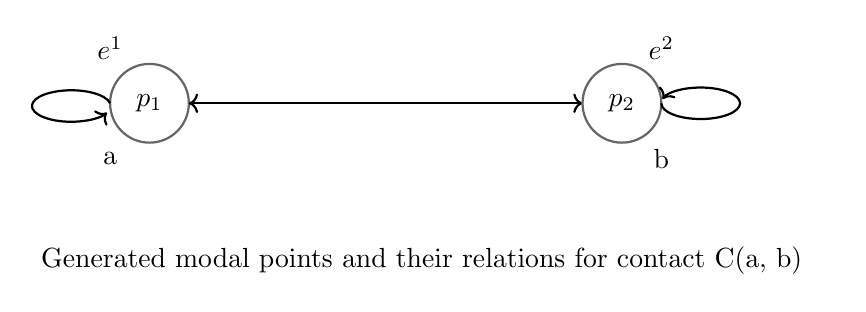
\begin{tikzpicture}[scale = 1]
		\filldraw[color=black!60, fill=red!0, thick](-3,0) circle (0.5);
		\node at (-3.5,0.7) {$\curvedE^1$};
		\node at (-3,0) {$p_1$};
		\node at (-3.5,-0.7) {a};
		\draw[thick, ->] (-3.5,0) arc [
      	  		start angle=10,
		       end angle=335,
        		x radius=0.5cm,
        		y radius =0.2cm
    			] ;
		\draw[thick, <->](-2.5,0) -- (2.5,0);
		\filldraw[color=black!60, fill=red!0, thick](3,0) circle (0.5);
		\node at (3.5,0.7) {$\curvedE^2$};
		\node at (3,0) {$p_2$};
		\node at (3.5,-0.7) {b};
		\draw[thick, ->] (3.5,0) arc [
      	  		start angle=180,
		      end angle=525,
        		x radius=0.5cm,
        		y radius =0.2cm
    			] ;
		\node[text width=10cm, anchor=west, right] at (-4.5,-2)
    		{Generated modal points and their relations for contact C(a, b)};
      \end{tikzpicture}
	\end{center}

	\begin{defn}\label{def-non-zero-construction}
		Let B be a branch conjunction and $a \neq 0 \in B$, where a is a term. Then one modal point p is generated and its variable valuations $\curvedE$ such that:
		\begin{itemize}
			\item $\vBool_{\curvedE}(a) = \textbf{true}$
		\end{itemize}
		The R relation is extended as follows:
		\begin{itemize}
			\item $pRp$ - reflexivity of the modal point $p$
		\end{itemize}
	\end{defn}
	\leavevmode\newline
	The constructed point diagram:
	\begin{center}
	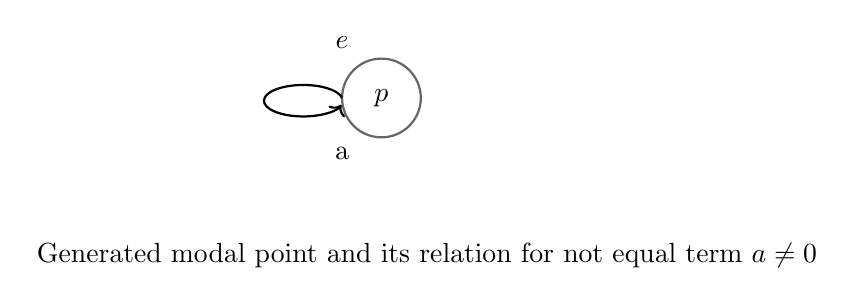
\begin{tikzpicture}[scale = 1]
		\filldraw[color=black!60, fill=red!0, thick](-0,0) circle (0.5);
		\draw[thick, ->] (-0.5,0) arc [
      	  		start angle=10,
		       end angle=345,
        		x radius=0.5cm,
        		y radius =0.2cm
    			] ;
		\node at (-0.5,0.7) {$\curvedE$};
		\node at (-0,0) {$p$};
		\node at (-0.5,-0.7) {a};
		\node[text width=10cm, anchor=west, right] at (-4.5,-2)
    		{Generated modal point and its relation for not equal term $a \neq 0$};
      \end{tikzpicture}
	\end{center}
	With definition \ref{def-non-zero-construction} the constructed model satisfies the non zero terms from the branch conjunction. \\
	With definition \ref{def-contacts-construction} the constructed model satisfies the contacts and the symmetric property of the non contacts from the branch conjunction. \\
	A model constructed with definitions \ref{def-non-zero-construction} and \ref{def-contacts-construction} will be denoted as a \textbf{partial model}. The points in the partial model are represented with a tuple $\langle \curvedE, a \rangle$.
           Furthermore, it must be verified that each of the modeled <$\curvedE$, a> modal point satisfies the equal to zero terms and the reflexivity of the non contacts from the branch conjunction.

	\begin{defn}
		Let M be a partial model. Then we say that the partial model M satisfies an equal to zero term $a = 0$, if the following holds:
		\begin{align*}
			\forall \langle \curvedE, a \rangle \in M: \vBool_{\curvedE}(a) = \textit{false}
		\end{align*}
	\end{defn}

	\begin{defn}
		Let M be a partial model. Then we say that the partial model M satisfies the reflexivity of a non contact $\neg C(a, b)$, if the following holds:
		\begin{align*}
			\forall \langle \curvedE, a\rangle \in M: \vBool_{\curvedE}(a) = false \lor \vBool_{\curvedE}(b) = false
		\end{align*}
	\end{defn}		

	\begin{defn}
		Let M be a partial model and let $\Ts$ be the set of all terms. Then the model valuation $\vE : \Ts \rightarrow \mathscr{P}(W)$ is defined inductively as:
		\begin{itemize}
			\item $\vE(0) = W$
			\item $\vE(1) = \emptyset$
			\item $\vE(p) = \{ \langle \curvedE, a \rangle \; | \; \langle \curvedE, a \rangle \in W \:\:\textit{and}\:\: \curvedE(p) = \textit{true}$
			\item $\vE(a \sqcap b) = \vE(a) \cap \vE(b)$
			\item $\vE(a \sqcup b) = \vE(a) \cup \vE(b)$
			\item $\vE(a*) = W \setminus \vE(a)$
		\end{itemize}
	\end{defn}
		The tuple $(W, R, \vE)$ is called a potential model.

	\leavevmode\newline
	To validate that the potential model is correct, meaning that it satisfies the formula, we must take into account the measure atomic formulas. 
	In order to satisfy the measure atomic formulas, additional points are generated and have the following structure $\langle \curvedE, 1 \rangle$. This means that 
	for each modal point the constant term 1 is taken together with a variable evaluation function. The variable evaluation functions of these modal points 
	is chosen such that the model satisfies all measure atomic formulas.

	\begin{defn}
		Let B be a branch conjunction and let N be the number of all measure atomic formulas ( $\le_\mu$ and $\leq_\mu$).
		Then N additional modal points are generated in the potential model \{$\langle \curvedE_i, 1 \rangle : 0 < i \leq N$ \}. The variable evaluation of the generated points must satisfy the measure atomic formulas.
		Satisfying a set of measure atomic formulas produces a system of inequalities.
	\end{defn}

	\subsection{System of Inequalities} 
		The system of inequality has the following structure:
		\[
			\syslineskipcoeff{1.50}
			\systeme*{\sum_{i^1} X_{i^1} <= \sum_{j^1} X_{j^1},
				\:\:.\:\:.\:\:.,
				\sum_{i^n} X_{i^n} <= \sum_{j^n} X_{j^n}, 
				\sum_{k^1} X_{k^1} > \sum_{l^1} X_{l^1},
				\:\:.\:\:.\:\:.,
				\sum_{k^m} X_{k^m} > \sum_{l^m} X_{l^m}
				}
		\]

		\leavevmode\newline
		\subsection{System Construction}
		Let $M = (W, R, \vE)$ be a potential model. The system of inequalities is constructed from the potential model by evaluating each
		of the terms in the $\le_\mu$ and $<_\mu$ atomic formulas. The number of points in the model are $N = | \; W \; |$. Let us enumerate the points
		$p_0, p_1, ..., p_N$. The system will have N different variables $X_0, X_1, ..., X_N$, 
		where $\forall i < N: X_i \textit{ is mapped to point }p_i$.

		\begin{defn}
			Let x and y be two terms, then the formula $\le_\mu(x, y)$ is transformed to an inequality as follows:
			\begin{align*}
				\sum_{i \in \vE(x)} X_i <= \sum_{j \in \vE(y)} X_j
			\end{align*}
		\end{defn}

		\begin{defn}
			Let x and y be two terms, then the formula $<_\mu(x, y)$ is transformed to an inequality as follows:
			\begin{align*}
				\sum_{i \in \vE(x)} X_i < \sum_{j \in \vE(y)} X_j
			\end{align*}
		\end{defn}

		\begin{defn}
			Let x and y be two terms and let $\mathscr{I}_q$ be the inequality produced from $\le_\mu(x, y)$. Then the inequality $\mathscr{L}_q$ can be simplified 
			by removing all variables present on both sides of the equation. This can be written as:
			\begin{align*}
				\sum_{i \in \vE(x) \setminus \vE(y)} X_i <= \sum_{j \in \vE(y) \setminus \vE(x)} X_j
			\end{align*}
		\end{defn}

		\begin{defn}
			Let x and y be two terms and let $\mathscr{I}_q$ be the inequality produced from $<_\mu(x, y)$. Then the inequality $\mathscr{L}_q$ can be simplified 
			by removing all variables present on both sides of the equation. This can be written as:
			\begin{align*}
				\sum_{i \in \vE(x) \setminus \vE(y)} X_i < \sum_{j \in \vE(y) \setminus \vE(x)} X_j
			\end{align*}
		\end{defn}

		\begin{defn}
			Let $M = (W, R, \vE)$ be a potential model. Let $\mathscr{S}$ be the system of inequalities defined by
			\begin{itemize}
				\item inequalities for all $\le_\mu$ fromulas by def: 3.16 
				\item inequalities for all $<_\mu$ fromulas by def: 3.17
				\item inequality $0 < X_i$ for each $0 \le i < N$  
			\end{itemize}
			If the system of inequalities $\mathscr{S}$ has a solution, then we say that the system is valid.
		\end{defn}
		\begin{lemma}
			\label{building-lemma}
			Let $\varphi$ be a formula. If there exists branch conjunction B for the formula $\varphi$
			and there exists a potential model M for the branch conjunction B and 
			there exists a valid system of inequalities defined from the potential model M,
			then the formula $\varphi$ is satisfiable by the model M.
		\end{lemma}

	\newpage
	\section{Implementation Introduction}
	The main programming language is C++. Flex \& Bison are used to parse the input formula. The formula prover is a C++ library. The unit and performance tests are C++ applications.
	The user application is a Web page. The Web server is implemented with the third party CppRestSDK library. The satisfiability checking runs on the server. There is a feature to interrupt an ongoing process. Can be triggered by the user via a button. There is a user disconnecting detection which cancels the requested formula proving. \\
	The project repository is at:

	\url{https://github.com/Anton94/modal_logic_formula_prover}. \\
	Each commit is build and tested on a various compilers (Windows and Linux OS).
		
	\subsection{Syntax}
	The formula should be easy and intuitive to write. Only the keyboard keys should be used. The legend below describes the formula's syntax:

	\begin{center}
	\begin{tabular}{ |c|c|c| }
		\hline
		\multicolumn{3}{|c|}{\textbf{Terms}} \\
		\hline
		0 				    & 0      & Boolean constant 0 \\
		1 					& 1      & Boolean constant 1 \\
		- 					& *      & Boolean complement \\
		*				 	& $\cap$ & Boolean meat \\
		+ 					& $\cup$ & Boolean join \\
		()                  & ()     & Parentheses \\
		\text{[a-zA-Z0-9]+} & $x_1$  & Boolean variable. Syntax $x1$, $Y42$, $Var101$ \\
		\hline
		\hline
		\multicolumn{3}{|c|}{\textbf{Formulas}} \\
		\hline
		F      & $\bot$            & Propositional constant false \\
		T      & $\top$            & Propositional constant true \\
		$\sim$ & $\neg$            & Negation \\
		$\&$   & $\land$           & Conjunction \\
		$|$    & $\lor$            & Disjunction \\
		->     & $\Rightarrow$     & Implication \\
		<->    & $\Leftrightarrow$ & Equivalence \\
		C      & C                 & Contact, syntax C($t_1$, $t_2$) \\
		<=     & $\leq$            & Part of , syntax <=($t_1$, $t_2$) \\
		<=m    & $\leq$$m$$$       & Measured Part of, syntax <=m($t_1$, $t_2$) \\
		=0     & =0                & Zero term, syntax $t_1=0$ \\
		()     & ()                & Parentheses \\
		\hline
	\end{tabular}
	\end{center}

	These are a few examples of formulas:
	\begin{itemize}
		\item $C(x1 * 1, x2 + y1)$
		\item $C(x1 + 0, (-x2 + x3) * x1)$
		\item $C(x1,x2) \;\&\; C(x2, x3) \;\& \sim C(x1,x3)$
		\item $C(x1,x2) \;\& <=(x1,x3) \;\& \sim C(x2,x3)$
		\item $C(x1,x2) \text{ -> } C(x2, x1)$
		\item $C(x1,x2) \;\&\; C(x2, x3) => C(x1, x3)$
		\item $F \text{ -> } C(x1,x2) \;\& \sim C(x1,x2)$
	\end{itemize}

	\subsection{Formula parsing}
	The formula is a sequence of characters. These characters do not give us any information for the formula's structure. It should be analyzed. Flex \cite{flex-tokenizer} and Bison \cite{bison-parser} are used to parse it into an AST (Abstract Syntax Tree). Flex is used as a tokenizer. Bison is used as the parser.

	\subsubsection{Abstract Syntax Tree}
	The AST is a binary tree. Each node has an operation type and up to two children. The formula nodes are prior term nodes. A formula node could have term node as children. Term nodes could not have a formula node as a child. The leaves are variables or constants.
	
	Let $\phi = (C(x1,x2) \;\& <=(x2, x3)) => C(x1, x3)$. The following is an AST of $\phi$:

\begin{tikzpicture}[
  tlabel/.style={pos=0.6,right=-1pt,font=\footnotesize\color{red!70!black}},
]
\label{AST-phi}
\node{=>}
child {node {$\&$}
  child {node {C}
    child {node {x1}}
    child {node {x2}}
  }
  child[missing] {}
  child {node {<=}
    child {node {x2}}
    child {node {x3}}
  }
}
child[missing] {}
child[missing] {}
child {node {C}
  child {node {x1}}
  child {node {x3}}
};
\end{tikzpicture}

	\newpage
	\paragraph{Operation types} Enum structure is used to represent the type of formulas and terms in a memory efficient way.
	\\
	\\
\noindent
\textit{ast.h}
	\begin{lstlisting}[language=C++]
enum class formula_operation_t
{
    constant_true,
    constant_false,
    conjunction,
    disjunction,
    negation,
    implication,
    equality,
    contact,
    less_eq,
    measured_less_eq,
    eq_zero
};

enum class term_operation_t
{
    constant_true,
    constant_false,
    union_, // union is a keyword
    intersection,
    complement,
    variable
};
	\end{lstlisting}

	\newpage
	\paragraph{Node types} There are two types of nodes. Formula nodes and term nodes. They are defined with a separate classes.
	\\
	\\
\noindent
\textit{ast.h}
	\begin{lstlisting}
class Node
{
    ...
};

class NFormula : public Node
{
public:
    NFormula(formula_operation_t op,
             Node* left = nullptr, Node* right = nullptr);
    ...

    formula_operation_t op;
    Node* left;
    Node* right;
};

class NTerm : public Node
{
public:
    NTerm(term_operation_t op,
          NTerm* left = nullptr, NTerm* right = nullptr);
    ...

    term_operation_t op;
    NTerm* left;
    NTerm* right;
    std::string variable;
};
	\end{lstlisting}

	\subsubsection{Tokenizer}
	The tokenizer is responsible for demarcating the special symbols in the input formula.
	After the symbols are identified, a token is created for each of them, or at least for those significant to the semantic of the input formula.
	For example, the whitespace is not significant, and a token is not created for them.
	We shall use Flex as a tokenizer \cite{flex-tokenizer}.

	\paragraph{Grammar} The tokenizer's grammar is composed of two types of tokens. Single character and multi character.

	The Single character tokens are directly matched in the input formula and are representing the token itself.
	The multi character token is a sequence of characters which have some meaning when bundled together.
	This tokenizer's grammar is unambiguous, and each input formula is uniquely tokenized.

	The tokens' derivation is explained in details in the following table with Flex syntax. The matched symbol represents the symbol from the input formula, and the output token is the newly created token for the matched symbol.

		\begin{flushleft}
			\centering
			\begin{tabular}{ | m{10em} | m{15em}| } 
				\hline
					\textbf{Matched sequence} & \textbf{Output token} \\ [0.7ex] 
				\hline
					[ \textbackslash t\textbackslash  n] & ; \\
				\hline
					[,TF01()C\&|~*+-] 	& yytext[0];  \\
				\hline
				    "<="            &   T\_LESS\_EQ; \\
				\hline
				    "<=m"           &   T\_MEASURED\_LESS\_EQ; \\
				\hline
				    "= 0"           &   T\_EQ\_ZERO; \\
				\hline
				    "->"            &   T\_FORMULA\_OP\_IMPLICATION; \\
				\hline
				    "<->"           &   T\_FORMULA\_OP\_EQUALITY; \\
				\hline
				    [a-zA-Z0-9]+    &   T\_STRING; \\
				\hline
				    .               &   yytext[0]; \\
				\hline
			\end{tabular}
		\end{flushleft}
	Let us review the table above. All white spaces, tabulations and newlines are ignored. The syntax for it is the \textbf{;} character.

	All single character tokens are passed as their ASCII code. The syntax for it is \textbf{yytext[0]}. It gives the matched character. That way, it will be easy to use them in the parser.

	The multi character tokens are converted to unique identifiers. For example, the "<=" sequence is converted to T\_LESS\_EQ. The sequence of letters and numbers is converted to T\_STRING. Later, it will be used as a term variable.

	The last matched symbol in the table represents everything else, if nothing has been matched then just return the text itself.
	The parser will use it to prompt where the unrecognized symbol was found, and the symbol itself can be printed out.

% Returns T\_STRING literal type and the string  value is written to yylval which can be later accessed from the parser. Note that it uses our simple memory manager to allocate this string in order to be able to safely free all allocated strings even when some syntax error occurs 

	\subsubsection{Parser}
			The single character tokens are passed as their ASCII symbol to Bison. 
			As discussed above, the multi character tokens need more clearance in order to represent the literal from the input text symbols.
			The followings are definition of literals for multi character tokens:
			\begin{itemize}
				\item \%token <const char*> T\_STRING is the literal for "string"
				\item \%token T\_LESS\_EQ is the literal for "<="
				\item \%token T\_MEASURED\_LESS\_EQ is the literal for "<=m"
				\item \%token T\_EQ\_ZERO is the literal for "=0"
				\item \%token T\_FORMULA\_OP\_IMPLICATION is the literal for "->"
				\item \%token T\_FORMULA\_OP\_EQUALITY is the literal for "<->"
			\end{itemize}
			The followings are definitions of priority and associativity of the operation tokens. 
			The priority is from low to high (w.r.t. the line order in which they are defined)
			\begin{itemize}
				\item \%left T\_FORMULA\_OP\_IMPLICATION T\_FORMULA\_OP\_EQUALITY
				\item \%left '|' '+'
				\item \%left '\&' '*'
				\item \%right '\textasciitilde' '-'
				\item \%nonassoc '(' ')'
			\end{itemize}

		\paragraph{Grammar}
			With the usage of the Parser literals, the input formula can be parsed to an Abstract Syntax Tree(AST).
			The AST contains all the data from the input string formula in a more structured way.
			On the AST additional optimizations can be done which will simplify the initial formula. It will produce better performance when a model is sought in the satisfiability algorithms.

			For convenience, will define two helper methods. Namely, \textbf{create\_term\_node} and \textbf{create\_formula\_node}. Both method construct AST nodes.

			The create\_term\_node method creates an AST term node. Its arguments are an operation and up to two child terms. Depending on the operation arity.

			The create\_formula\_node is analogous to the create\_term\_node method. Creates an AST formula node.

			Few special symbols to define beforehand:
			\begin{itemize}
				\item \textbf{\$\$} is the return value to the 'parent'. Later, he can use it, e.g. as a child.
				\item \textbf{\$i} is the return value of the i-th matched element in the matcher sequence.
			\end{itemize}

		\paragraph{Algorithm} The following is the parser algorithm, which produces an Abstract Syntax Tree.
	\\
	\\
\noindent
\textit{parser.y}
	\begin{lstlisting}
formula // 'formula' non-terminal
    : 'T' { // matching token 'T'
        $$ = create_formula_node(constant_true);   
    }
    | 'F' {
        $$ = create_formula_node(constant_false);
    }
    | 'C' '(' term ',' term ')' {
        $$ = create_formula_node(contact, $3, $5); 
    }
    | "<=" '(' term ',' term ')' {
        $$ = create_formula_node(less_eq, $3, $5);
    }
    | "<=m" '(' term ',' term ')' {
        $$ = create_formula_node(measured_less_eq, $3, $5);
    }
    | term "=0" {
        $$ = create_formula_node(eq_zero, $1);
    }
    | '(' formula '&' formula ')' {
        $$ = create_formula_node(conjunction, $2, $4);
    }
    | formula '&' formula {
        $$ = create_formula_node(conjunction, $1, $3);
    }
    | '(' formula '|' formula ')' {
        $$ = create_formula_node(disjunction, $2, $4);
    }
    | formula '|' formula {
        $$ = create_formula_node(disjunction, $1, $3);
    }
    | '~' formula {
        $$ = create_formula_node(negation, $2);
    }
    | '(' formula "->" formula ')' {
        $$ = create_formula_node(implication, $2, $4);
    }
    | formula "->" formula {
        $$ = create_formula_node(implication, $1, $3);
    }
    | '(' formula "<->" formula ')' {
        $$ = create_formula_node(equality, $2, $4);
    }
    | formula "<->" formula {
        $$ = create_formula_node(equality, $1, $3);
    }
    | '(' formula ')' {
        $$ = $2;
    }
  ;
term
    : '1' {
        $$ = create_term_node(constant_true);
    }
    | '0' {
        $$ = create_term_node(constant_false);
    }
    | "string" {
        $$ = create_term_node(term_operation_t::variable);
        $$->variable = std::move(*$1);
        // the string is allocated from the
        // tokenizer and we need to free it
        free_lexer_string($1); 
    }
    | '(' term '*' term ')' {
        $$ = create_term_node(intersection, $2, $4);
    }
    | term '*' term {
        $$ = create_term_node(intersection, $1, $3);
    }
    | '(' term '+' term ')' {
        $$ = create_term_node(union_, $2, $4);
    }
    | term '+' term {
        $$ = create_term_node(union_, $1, $3);
    }
    | '-' term {
        $$ = create_term_node(complement, $2);
    }
    | '(' term ')' {
        $$ = $2;
    }
  ;
	\end{lstlisting}

	\subsection{Formula refinement}
	The AST can be easily modified and optimized. One of the modifications is removing the implications and equivalences. They are replaced by conjunction, disjunction and negation. This is convenient because it simplifies the tableau method. It does not have to handle implication and equivalence operations. The following is a modified AST of $\phi$ \ref{AST-phi} without the implication:
	
\begin{tikzpicture}[
  tlabel/.style={pos=0.6,right=-1pt,font=\footnotesize\color{red!70!black}},
]
\node{$|$}
child {node {$\sim$}
  child {node {$\&$}
    child {node {C}
      child {node {x1}}
      child {node {x2}}
    }
    child[missing] {}
    child {node {<=}
      child {node {x2}}
      child {node {x3}}
    }
  }
}
child[missing] {}
child[missing] {}
child {node {C}
  child {node {x1}}
  child {node {x3}}
};
\end{tikzpicture}

	\subsubsection{Visitor Pattern} The AST modification is best achieved with the visitor pattern \cite{visitor-pattern}. Uses double virtual dispatching. Separates the algorithm from the object structure on which it operates. Allows new visitors to be added in a simple manner. Each AST modification will be implemented as a visitor. Will not explain the pattern in depth. In essence, the visitor pattern requires the AST nodes to implement a virtual \textbf{accept} method. This method accepts a visitor as argument and calls the visitor's virtual \textbf{visit} method with the real node's type. This is the double virtual dispatching. One virtual call to find the node's real type. Another to find the visitor's real type. Now, adding a new visitor requires only adding its class. Does not require changes in the AST node classes or other visitor classes.

\newpage
\noindent
\textit{visitor.h}
\begin{lstlisting}
...
class Visitor
{
public:
    virtual void visit(NFormula& f) = 0;
    virtual void visit(NTerm& t) = 0;
};

// Example visitor(aglorithm) which will print the AST tree.
class VPrinter : public Visitor
{
public:
    void visit(NFormula& f) override
    {
        // Print the formula node's data.
    }
    void visit(NTerm& t) override
    {
        // Print the term node's data.
    }
};

class Node
{
public:
    virtual void accept(Visitor& v) = 0;
};

class NFormula : public Node
{
public:
    void accept(Visitor& v) override { v.visit(*this); }

    ...
};

class NTerm : public Node
{
public:
    void accept(Visitor& v) override { v.visit(*this); }

    ...
};
\end{lstlisting}

	\newpage
	It's worth showing the implementation of the VPrinter visit methods. They are simple and a good illustration of the pattern. Shows how the AST tree is traversed by calling the VPrinter instance with the AST's root node.	
	\\
	\\
\noindent
\textit{visitor.cpp}
\begin{lstlisting}
void VPrinter::visit(NFormula& f)
{
    switch(f.op)
    {
        case formula_operation_t::constant_true:
            out_ << "T"; // out_ is an output stream, e.g. std::cout.
            break;
        case formula_operation_t::constant_false:
            out_ << "F";
            break;
        case formula_operation_t::conjunction:
            out_ << "(";
            f.left->accept(*this);
            out_ << " & ";
            f.right->accept(*this);
            out_ << ")";
            break;
        case formula_operation_t::disjunction:
            // Analogous to conjunction. The symbol is '|'.
        case formula_operation_t::implication:
            // Analogous to conjunction. The symbol is '->'.
        case formula_operation_t::equality:
            // Analogous to conjunction. The symbol is '<->'.
        case formula_operation_t::negation:
            out_ << "~";
            f.left->accept(*this);
            break;
        case formula_operation_t::less_eq:
            out_ << "<=(";
            f.left->accept(*this);
            out_ << ", ";
            f.right->accept(*this);
            out_ << ")";
            break;
        case formula_operation_t::measured_less_eq:
            out_ << "<=m(";
            f.left->accept(*this);
            out_ << ", ";
            f.right->accept(*this);
            out_ << ")";
            break;
        case formula_operation_t::eq_zero:
            out_ << "(";
            f.left->accept(*this);
            out_ << ")=0";
            break;
        case formula_operation_t::contact:
            out_ << "C(";
            f.left->accept(*this);
            out_ << ", ";
            f.right->accept(*this);
            out_ << ")";
            break;
        default:
            assert(false && "Unrecognized.");
    }
}

void VPrinter::visit(NTerm& t)
{
    switch(t.op)
    {
        case term_operation_t::constant_true:
            out_ << "1";
            break;
        case term_operation_t::constant_false:
            out_ << "0";
            break;
        case term_operation_t::variable:
            out_ << t.variable;
            break;
        case term_operation_t::union_:
            out_ << "(";
            t.left->accept(*this);
            out_ << " + ";
            t.right->accept(*this);
            out_ << ")";
            break;
        case term_operation_t::intersection:
            // Analogous to union_. The symbol is '*'.
        case term_operation_t::complement:
            out_ << "-";
            t.left->accept(*this);
            break;
        default:
            assert(false && "Unrecognized.");
    }
}
\end{lstlisting}

	\subsubsection{Visitors Overview}
	The following are the supported visitors. Their implementation is close to a thousand lines of code and can be checked in the repository.
	\paragraph{VReduceConstants}
	Removes all unnecessary children of And/Or/Negation operations of the following type:
			\begin{table}[H]
				  \centering
				  \begin{tabular}{llll}
				    \toprule
				    \midrule
				\tabitem \textasciitilde T $\equiv$ F & \tabitem C(0,0)  $\equiv$ F & \tabitem \textasciitilde F $\equiv$ T & \tabitem C(1,1) $\equiv$ T \\
				\tabitem (T \& T) $\equiv$ T & \tabitem C(a,0)  $\equiv$ F & \tabitem (F | F) $\equiv$ F & \tabitem C(0,a) $\equiv$ F \\
				\tabitem (g \& T) $\equiv$ g & \tabitem -1 $\equiv$ 0 & \tabitem (g | T) $\equiv$ T & \tabitem -0 $\equiv$ 1 \\
				\tabitem (T \& g) $\equiv$ g & \tabitem (1 * 1) $\equiv$ 1 & \tabitem (T | g) $\equiv$ T & \tabitem (0 + 0) $\equiv$ 0 \\
				\tabitem (g \& F) $\equiv$ F & \tabitem (t * 1) $\equiv$ t & \tabitem (g | F) $\equiv$ g & \tabitem (t + 1) $\equiv$ 1 \\
				\tabitem (F \& g) $\equiv$ F & \tabitem (1 * t) $\equiv$ t & \tabitem (F | g) $\equiv$ g & \tabitem (1 + t) $\equiv$ 1 \\
				\tabitem 0=0 $\equiv$ T & \tabitem (t * 0) $\equiv$ 0 & \tabitem 1=0 $\equiv$ F & \tabitem (t + 0) $\equiv$ t \\
				\tabitem <=(0,a) $\equiv$ T & \tabitem (0 * t) $\equiv$ 0 & \tabitem <=(a,1) $\equiv$ T & \tabitem (0 + t) $\equiv$ t \\

					    \bottomrule
				  \end{tabular}
				\end{table}

	\paragraph{VConvertContactsWithConstantTerms}
				Converts C with constant 1 terms in !=0 atomic formulas.
				This visitor is best used after the contacts are reduced, via VReduceConstants
				\begin{itemize}
					\item C(a,1) $\equiv$ \textasciitilde(a=0)
					\item C(1,a) $\equiv$ \textasciitilde(a=0)
				\end{itemize}

	\paragraph{VConvertLessEqContactWithEqualTerms}
				Converts C and <= atomic formulas with identical terms:
				\begin{itemize}
					\item <=(a,a) $\equiv$ T, \\
						since (a * -a = 0))
					\item C(a,a) $\equiv$ \textasciitilde(a=0)
				\end{itemize}

	\paragraph{VReduceDoubleNegation}
				Removes the double/tripple/etc negations.
				This visitor is best used after all visitors which might add additional negations!
				\begin{itemize}
					\item -(-g) $\equiv$ g
					\item -(-t) $\equiv$ t
				\end{itemize}

	\paragraph{VConvertImplicationEqualityToConjDisj}
				Converts all formula nodes of type implication and equality to nodes
				which are using just conjunction and disjunction. The main reason for this visitor is to simplify the formula operations.
				This visitor simplifies the formula to contain only conjunctions, disjunctions and negation operations.
				\begin{itemize}
					\item (f -> g)  $\equiv$ (\textasciitilde f | g)
					\item (f <-> g) $\equiv$ ((f \& g) | (\textasciitilde f \& \textasciitilde g))
				\end{itemize}

	\paragraph{VConvertLessEqToEqZero}
				Converts a <= formula to an equal to zero atomic formula
				\begin{itemize}
					\item <=(a,b) $\equiv$ (a * -b) = 0
				\end{itemize}

	\paragraph{VSplitDisjInLessEqAndContacts}
				Divides C and <= atomic formulas with a disjunction term into two simpler formulas
				\begin{itemize}
					\item C(a + b, c) $\equiv$ C(a, c) | C(b, c)
					\item C(a, b + c) $\equiv$ C(a, b) | C(a, c)
					\item <=(a + b, c) $\equiv$ <=(a,c) \& <=(b,c)
				\end{itemize}

	There are few visitors which only collect or print information from the formula
				\begin{itemize}
					\item VVariablesGetter - gets all variables from the formula (as string)
					\item VPrinter - prints the formula to some provided output stream
				\end{itemize}

	\subsection{Formula building}
	The formula is a binary tree. A \textbf{subformula} is a subtree in the formula's tree. The process of building a satisfiable model is computational heavy. A part of it is lexical comparing and traversing subformulas. The AST is convenient to modify the formula. These modifications are a preprocessing step. After them, the formula will not be modified. A few optimizations could be done.

	\subsubsection{Optimizations}
	\paragraph{Reducing formula operations}
	The formula operations could be reduced to not have \textit{implication}, \textit{equivalence} and \textit{less equal}. The \textit{VConvertImplicationEqualityToConjDisj} and \textit{VConvertLessEqToEqZero} visitor should be applied.

	\paragraph{Variable substitution}
	The variables are a sequence of characters, i.e. strings. It is slow to compare them. An integer ID could be assigned to each variable. One way to do it is via the \textit{VVariablesGetter} visitor. Retrieve all unique variables in a vector and use their positions as IDs.

	\paragraph{Hashing subformulas}
	Conducting a test whether two subformulas are equal in a lexical way is an important procedure for the sake of performance. Such equality checks are required in various situations. One of which is checking if a subformula exists in a set of subformulas.

	Have in mind that the naive solution to do an equality check is to compare the whole subformula structure. The complexity is O(n), where n is the size of the subformula. To reduce this complexity, a precalculated hash value shall be used.
	For each formula node an additional hash variable is stored. The hash is computed recursively through the formula's structure. The hash of a parent node depends on the hashes of its children nodes. 
	The equality comparison first checks the hash codes. The full equality checking is done only for matching hash codes.

	\newpage
	\subsubsection{Layout}
	The formula structure will be similar to the AST. A couple of changes reflecting the optimizations above. The following is the final formula node's layout.
	\\
	\\
\noindent
\textit{formula.h} / \textit{term.h}
\begin{lstlisting}
class formula {
    ...
    enum class operation_type : char {
        constant_true,
        constant_false,
        conjunction,
        disjunction,
        negation,
        measured_less_eq,
        eq_zero,
        c,
        invalid,
    };

    operation_type op_;
    std::size_t hash_;

    struct child_formulas {
        formula* left;
        formula* right;
    };
    struct child_terms {
        term* left;
        term* right;
    };

    union {
        // Holds only one of the described objects.
        // Depending on the operation type the
        // child_f_ or child_t_ is "valid".
        child_formulas child_f_;
        child_terms child_t_;
    };
};

class term {
    ...
    enum class operation_type : char
    {
        constant_true,
        constant_false,
        union_,
        intersection,
        complement,
        variable,
        invalid,
    };

    operation_type op_;
    std::size_t hash_;

    struct children
    {
        term* left;
        term* right;
    };
    union {
        // Holds either children or variable id.
        // Depending on the node's operation type.
        children children_;
        size_t variable_id_;
    };
};
\end{lstlisting}

	\subsubsection{Hashing}
	The following is the implemented hash construction procedure for the term node. The formula node is analogous.
	\\
	\\
\noindent
\textit{term.h}
\begin{lstlisting}
void term::construct_hash()
{
  switch(op_)
  {
  case operation_t::constant_true:
  case operation_t::constant_false:
    break;
  case operation_t::union_:
  case operation_t::intersection:
    hash_ = ((children.left->get_hash() & 0xFFFFFFFF) * 2654435761) +
        children.right->get_hash() & 0xFFFFFFFF) * 2654435741);
    break;
  case operation_t::complement:
    hash_ = (children.left->get_hash() & 0xFFFFFFFF) * 2654435761;
    break;
  case operation_t::variable:
    hash_ = (variable_id_ & 0xFFFFFFFF) * 2654435761;
    break;
  default:
    assert(false && "Unrecognized.");
  }

  // Add the operation type to the hash.
  const auto op_code = static_cast<unsigned>(op_) + 1;
  hash_ += (op_code & 0xFFFFFFFF) * 2654435723;
}
\end{lstlisting}

	Let $\tau_1$ and $\tau_2$ be two terms. Let $h_1$ be the precalculated hash of $\tau_1$ and $h_2$ be the precalculated hash of $\tau_2$.
	The equality check procedure follows the following steps:
	\begin{itemize}
		\item if $h_1 \neq h_2$, then the terms are not equal
		\item if $h_1 = h_2$, then recursively compare the children.
	\end{itemize}
	\noindent

	\newpage
	\subsubsection{Conversion from AST}
	The formula building from an AST is straightforward. Recursive depth first iteration over the AST. For each AST node, a corresponding formula/term node is constructed. The implementation could be found in \textit{term.cpp} and \textit{formula.cpp} in the repository.

	\newpage
	\section{Tableaux Implementation}
	The Tableaux process is a decision procedure. Recursively breaks down a given formula into basic components. Based on that, a decision can be concluded. The recursive step breaks down a formula part into one or two subformulas. Continuously applying the recursive step produces a binary tree. The nodes are the formulas, and the links represent the recursive step.

	All formulas in a branch are considered to be in conjunction. Contradiction may arise in a same branch if there exists a formula and its negation.

	The main principle of the tableaux is to break a complex formula into smaller ones until complementary pairs of atomic formulas are produced.

	\begin{defn}
		A set of only signed formulas represents a signed formula set. The letter \textit{X} is usually used for its representation.
	\end{defn}

	\subsection{Tableaux Step}
	The \textit{Tableaux Step} takes as input a formula and a signed formulas set and produces as output one or two new formulas, depending on the operation.
	The signed formulas set consists of the broken down formulas by previous tableaux steps.
	The output of the tableaux step depends on the rule applied to the formula.

	\subsection{Rules}
	Only \textit{negation} \textit{conjunction} and \textit{disjunction} operations will be handled. The implication and equivalence are converted.

		\subsubsection*{Negation}
			$\begin{array}{rl}
				& \signT(\neg \varphi), X \\
			      \cline{2-2}
			      & \signF(\varphi), X
			\end{array}$
			\:\:\:\:\:\:\:\:\:\:\:\:\:\:\:\:\:\:\:\:\:\:\:\:\:\:\:\:\:\:\:\:\:\:\:\:\:\:\:\:\:\:\:\:\:\:\:\:
			$\begin{array}{rl}
				& \signF(\neg \varphi), X \\
			      \cline{2-2}
			      & \signT(\varphi), X
			\end{array}$

		\subsubsection*{Conjunction}
			$\begin{array}{rl}
				& \signT(\varphi \: \wedge \: \psi), X \\
			      \cline{2-2}
			      & \signT\varphi, \signT\psi, X
			\end{array}$
			\:\:\:\:\:\:\:\:\:\:\:\:\:\:\:\:\:\:\:\:\:\:\:\:\:\:\:\:\:\:\:\:\:\:\:
			$\begin{array}{rl}
				& \:\:\: \signF(\varphi \: \wedge \: \psi), X \\
			      \cline{2-2}
			      & \signF\varphi, X \:\:\:\:\:\:\:\: \signF\psi, X
			\end{array}$

		\subsubsection*{Disjunction}
			$\begin{array}{rl}
				& \:\:\: \signT(\varphi \: \vee \: \psi), X \\
			      \cline{2-2}
			      & \signT\varphi, X \:\:\:\:\:\:\:\: \signT\psi, X
			\end{array}$
			\:\:\:\:\:\:\:\:\:\:\:\:\:\:\:\:\:\:\:\:\:\:\:\:\:\:\:\:\:\:\:\:
			$\begin{array}{rl}
				& \signF(\varphi \: \vee \: \psi), X \\
			      \cline{2-2}
			      & \signF\varphi, \signF\psi, X
			\end{array}$

	\newpage
	For our case, the functionality of the tableaux process shall be extended. If the branch is not closed, there are additional calculations needed in order to verify that there is no contradiction. Namely, to verify that there is no contradiction on Term level. This means that there exists a satisfiable model.
	This verification can be done in different manners. Depending on the algorithm type. The best way to think about it is that the tableaux process returns a not-closed branch and if there is a model for the set of atomic formulas in this branch, then the formula is satisfiable, otherwise the tableaux process proceeds with the next not-closed branch. If such branch does not exist, then the formula is not satisfiable. 

	\subsection{Implementation}
	The program implementation of the tableaux method follows the standard tableaux process. The first interesting design decision is to keep all true signed formulas in one data set, and all false signed formulas in another data set. This enables fast searches whether a formula has been signed as true or false.

	\begin{defn}
	Let X be a set of formulas, then X is called \textbf{signed formula collection} if and only if all formulas in X are signed as true or all formulas are signed as false.
	\end{defn}

	This collection is implemented with \textit{std::unordered\_set} (hashset), which stores the formulas by pointers to their root nodes. The hashing uses the node's precalculated hash. The comparing is via the node's \textit{operator==}. That way, different pointers to subformulas with the same structure will be treated as identical.

	The average complexity for search, insert and erase in this collection is O(1). There is no formula copying. So, almost no memory overhead for keeping the formulas in the set.
	\newline
	\newline
	There are 8 signed formula collections:
%Note add definition for positive and negative collections !!!
	\begin{itemize}
		\item formulas\_T - contains only non-atomic formulas signed as true
		\item formulas\_F - contains only non-atomic formulas signed as false, \\
				For example, if $\neg\varphi$ is encountered as an output of the tableaux step, then only $\varphi$ is inserted into the formula\_F
		\item contacts\_T - contains only atomic contact formulas signed as true
		\item contacts\_F - contains only atomic contact formulas signed as false
		\item zero\_terms\_T - contains only formulas of type $\varphi \le \psi$ signed as true
		\item zero\_terms\_F - contains only formulas of type $\varphi \le \psi$ signed as false
		\item measured\_less\_eq\_T - contains only formulas of type $\varphi \le_m \psi$ signed as true
		\item measured\_less\_eq\_F - contains only formulas of type $\varphi \le_m \psi$ signed as false
	\end{itemize}

	These collections are unordered sets of points to the formulas/terms.
	\\
	\\
\noindent
\textit{types.h}
\begin{lstlisting}
using formulas_t = std::unordered_set<
	const formula*, 
	formula_ptr_hasher, 
	formula_ptr_comparator>;
using terms_t = std::unordered_set<
	const term*, 
	term_ptr_hasher, 
	term_ptr_comparator>;
\end{lstlisting}

\noindent
\textit{tableau.h}
\begin{lstlisting}
    formulas_t formulas_T_;
    formulas_t formulas_F_;
    formulas_t contacts_T_;
    formulas_t contacts_F_;
    terms_t zero_terms_T_;
    terms_t zero_terms_F_;
    formulas_t measured_less_eq_T_;
    formulas_t measured_less_eq_F_;
\end{lstlisting}

	\begin{defn}
	Let $\varphi$ be a signed formula, then $\varphi$ is causing a contradiction if any of the following is true:
	\begin{itemize}
		\item $\varphi$ is a non-atomic signed as true and $\varphi$ belongs to $formulas\_F$
		\item $\varphi$ is a non-atomic signed as false and $\varphi$ belongs to $formulas\_T$
		\item $\varphi$ is a contact formula signed as true and $\varphi$ belongs to $contacts\_F$
		\item $\varphi$ is a contact formula signed as false and $\varphi$ belongs to $contacts\_T$
		\item $\varphi$ is a zero terms formula signed as true and $\varphi$ belongs to $zero\_terms\_F$
		\item $\varphi$ is a zero terms formula signed as false and $\varphi$ belongs to $zero\_terms\_T$
		\item $\varphi$ is a measured less formula signed as true and $\varphi$ belongs to $measured\_less\_eq\_F$
		\item $\varphi$ is a measured less formula signed as false and $\varphi$ belongs to $measured\_less\_eq\_T$
	\end{itemize}
	\end{defn}
	\subsection*{Invariant}
	At any time, all formulas in all eight signed formula collections do not contradict.

	A contradiction may occur if a formula is split and some resulting components causes a contradiction.

	\subsubsection*{Example}
	Let's assume that $contacts\_T = \{ C(a, b)\}$ and let's have a look at the following formula $\signT(T \wedge \neg C(a,b))$.
	\newline
	By the rules of decomposition, namely the ( $\wedge$ ) rule produces $\signT T \text{ and } \signT\neg C(a,b)$.

	Then the $\signT\neg C(a,b)$ will be decomposed to $\signF C(a,b)$ by the ( $\neg$ ) rule, which causes a contradiction since $C(a,b)$ is already present in $contacts\_T$ formulas.

	\subsubsection*{Tableaux Algorithm}
	Given a formula $\varphi$, the following algorithm determines the atomic formulas in all branches of the tableaux process.

	As a first step if the formula $\varphi$ is the constant F, then false is returned directly, otherwise the whole formula $\varphi$ is inserted in $formulas\_T$.
	\newline
	\subsubsection*{Remarks}
	\begin{itemize}
		\item true boolean value is used to represent the formula constant T
		\item false boolean value is used to represent the formula constant F
		\item Contact atomic formula is commutative, meaning that: $C(a,b) \iff C(b,a)$
	\end{itemize}

	Few lemmas which will provide a much more efficient contradiction finding in the tableaux process.
	\subsubsection*{Emptiness Lemma}
	Let x be a term. Suppose that the atomic formula $x = 0$ has already been signed as true.
	Then marking the following formulas as true will lead to contradiction:
	\begin{itemize}
		\item C(x,y)
		\item C(y,x)
	\end{itemize}
	for any term y.

	\subsubsection*{Inverse Emptiness Lemma}
	Let x, y and z be terms. Suppose that the atomic formulas C(x,y) or C(z, x) has already been signed as true, then marking the formula x = 0 as true will lead to contradiction.
	\newline
	\subsubsection*{Time Complexity Emptiness Lemma and Inverse Emptiness Lemma}
	The algorithmic complexity to check whether a new formula leads to contradiction by Emptiness Lemma and Inverse Emptiness Lemma is done effectively. Namely, in constant time with the usage of one new collection $contact\_T\_terms\_$. It keeps the terms of the true contacts. Namely, the contacts in the collection $contacts\_T$. This means that for each $\signT(C(x, y))$, the terms x and y are in the mentioned collection of true terms. The $contact\_T\_terms\_$  is a multiset and keeps track of all added terms, meaning that if the term x is added twice and then removed only once, there will still be an entry of that x in the $contact\_T\_terms\_$ collection. Removing a true contact appears when moving up the tableau tree, i.e. switching to another branch.

	To check if a new formula leads to contradiction by Emptiness Lemma or Inverse Emptiness Lemma, the following method is used:
\begin{lstlisting}
auto has_broken_contact_rule(const formula* f) const -> bool;
\end{lstlisting}

	\subsection{Handy methods}
	\subsubsection*{Search for formula signed as true}
\begin{lstlisting}
auto find_in_T(const formula* f) const -> bool
\end{lstlisting}
	Checks existence of formula $\varphi$ in any positive collection depending on the type of $\varphi$. Namely, if $\varphi$ is of type:
	\begin{itemize}
		\item $C(x, y)$: returns whether $\varphi \in contacts\_T$
		\item $x = 0$: returns whether $\varphi \in zero\_terms\_T$
		\item $x \le_m y$: returns whether $\varphi \in measured\_less\_eq\_T$
		\item non-atomic formula: returns whether $\varphi \in formulas\_T$
	\end{itemize}

	\subsubsection*{Search for formula signed as false}
\begin{lstlisting}
auto find_in_F(const formula* f) const -> bool
\end{lstlisting}
	Checks existence of formula $\varphi$ in any negative collection depending on the type of $\varphi$. Namely, if $\varphi$ is of type:
	\begin{itemize}
		\item $C(x, y)$: returns whether $\varphi \in contacts\_F$
		\item $x = 0$: returns whether $\varphi \in zero\_terms\_F$
		\item $x \le_m y$: returns whether $\varphi \in measured\_less\_eq\_F$
		\item non-atomic formula: returns whether $\varphi \in formulas\_F$
	\end{itemize}

	\subsubsection*{Adding}
	\subsubsection*{Mark formula as true}
\begin{lstlisting}
void add_formula_to_T(const formula* f)
\end{lstlisting}
	Adds the formula $\varphi$ as true in in the respective positive collection. Namely, if $\varphi$ is of type:
	\begin{itemize}
		\item C(x, y): $\varphi$ is added to $contacts\_T$, and the terms x and y are added to the $contact\_T\_terms\_$
		\item $x = 0$: x is added in $zero\_terms\_T$
		\item $x \le_m y$: $\varphi$ is added to $measured\_less\_eq\_T$
		\item non-atomic formula: $\varphi$ is added to $formulas\_T$
	\end{itemize}

	\subsubsection*{Mark formula as false}
\begin{lstlisting}
void add_formula_to_F(const formula* f)
\end{lstlisting}
	Adds the formula $\varphi$ as false in the respective negative collection. Namely, if $\varphi$ is of type:
	\begin{itemize}
		\item C(x, y): $\varphi$ is added to $contacts\_F$
		\item $x = 0$: x is added in $zero\_terms\_F$
		\item $x \le_m y$: $\varphi$ is added to $measured\_less\_eq\_F$
		\item non-atomic formula: $\varphi$ is added to $formulas\_F$
	\end{itemize}

	\subsubsection*{Removing}
	\subsubsection*{Remove formula signed as true}
\begin{lstlisting}
void remove_formula_from_T(const formula* f)
\end{lstlisting}
	Removes the formula $\varphi$ from the respective positive collection. Namely if $\varphi$ is of type:
	\begin{itemize}
		\item C(x, y): $\varphi$ is removed from $contacts\_T$, and the terms x and y are removed from the $contact\_T\_terms\_$.
		\item $x = 0$: x is removed from $zero\_terms\_T$
		\item $x \le_m y$: $\varphi$ is removed from $measured\_less\_eq\_T$
		\item non-atomic formula: $\varphi$ is removed from $formulas\_T$
	\end{itemize}

	\subsubsection*{Remove formula signed as false}
\begin{lstlisting}
void remove_formula_from_F(const formula* f)
\end{lstlisting}
	Removes the formula $\varphi$ from the respective negative collection. Namely if $\varphi$ is of type:
	\begin{itemize}
		\item C(x, y): $\varphi$ is removed from $contacts\_F$
		\item $x = 0$: x is removed from $zero\_terms\_F$
		\item $x \le_m y$: $\varphi$ is removed from $measured\_less\_eq\_F$
		\item non-atomic formula: $\varphi$ is removed from $formulas\_F$
	\end{itemize}

	\newpage
	\subsection{Tableaux Satisfiable Step Implementation}
	The Tableaux satisfiable step is the whole Tableaux algorithm.
	\\
	\\
\noindent
\textit{tableau.cpp}
\begin{lstlisting}
auto tableau::satisfiable_step() -> bool
{
    // The bottom of the recursive algorithm is when we have
    // only atomic formulas(which does not contradicts).
    // Then we can run algorithms for model construction.
    if(formulas_T_.empty() && formulas_F_.empty())
    {
        // This is the method which tries
        // to construct satisfiable model.
        return has_satisfiable_model();
    }

    if(!formulas_T_.empty())
    {
        // Choosing some formula to handle in this step.
        // If this branch does not produce a valid satisfiable path,
        // then this formula will be returned to formulas_T_.
        auto f = *formulas_T_.begin();

        const auto op = f->get_operation_type();
        if(op == op_t::negation)
        {
            // T(~X) -> F(X)
            auto X = f->get_left_child_formula();
            if(X->is_constant())
            {
                // F(T) is not satisfiable
                if(X->is_constant_true())
                {
                    return false;
                }
                // F(F) is satisfiable, continue with the rest.
                return satisfiable_step();
            }

            if(find_in_T(X))
            {
                // Contradiction, we want to satisfy F(X)
                // but we already have to satisfy T(X).
                return false;
            }

            if(find_in_F(X)) // Skip adding F(X) multiple times.
            {
                return satisfiable_step();
            }

            add_formula_to_F(X);
            auto res = satisfiable_step();
            // Revert it on the way back.
            remove_formula_from_F(X);
            return res;
        }
\end{lstlisting}
\newpage
\begin{lstlisting}
        if(op == op_t::conjunction)
        {
            // T(X & Y) -> T(X) & T(Y)
            T_conjuction_child X(*this, f->get_left_child_formula());
            T_conjuction_child Y(*this, f->get_right_child_formula());

            // Checks if X breaks the contact rule
            // or brings a contradiction
            if(!X.validate())
            {
                return false;
            }
            X.add_to_T(); // Adds X to T collection

            if(!Y.validate())
            {
                X.remove_from_T();
                return false;
            }
            Y.add_to_T();

            auto res = satisfiable_step();
            X.remove_from_T();
            Y.remove_from_T();

            return res;
        }

        assert(op == op_t::disjunction);
        // T(X v Y) -> T(X) v T(Y)
        auto X = f->get_left_child_formula();
        auto Y = f->get_right_child_formula();
        trace() << "Will split to two subtrees: "
		<< *X << " and " << *Y;

        // T(T) is satisfiable and we can skip the other branch
        if(X->is_constant_true() || Y->is_constant_true())
        {
            trace() << "One of the childs is constant true";
            return satisfiable_step();
        }
\end{lstlisting}
\newpage
\begin{lstlisting}
        auto process_T_disj_child = [&](const formula* child) {
            if(child->is_constant_false() || // T(F) is not satisfiable
               find_in_F(child) || has_broken_contact_rule(child))
            {
                return false;
            }

            if(find_in_T(child)) // skip adding it multiple times
            {
                return satisfiable_step();
            }

            add_formula_to_T(child);
            const auto res = satisfiable_step();
            remove_formula_from_T(child);
            return res;
        };

        trace() << "Start of the left subtree: " << *X << " of " << *f;
        if(process_T_disj_child(X))
        {
            // There was no contradiction in the left path,
            // so there is no need to continue with the right path.
            return true;
        }

        trace() << "Start of the right subtree: " << *Y << " of " << *f;
        return process_T_disj_child(Y);
    }

    // Almost analogous but taking a formula from Fs

    // Choosing some formula to handle in this step.
    // If this branch does not produce a valid satisfiable path,
    // then this formula will be returned to formulas_F_
    auto f = *formulas_F_.begin();

    const auto op = f->get_operation_type();
    if(op == op_t::negation)
    {
        // F(~X) -> T(X)
        auto X = f->get_left_child_formula();
        if(X->is_constant())
        {
            // T(F) is not satisfiable
            if(X->is_constant_false())
            {
                return false;
            }
            // T(T) is satisfiable, continue with the rest
            return satisfiable_step();
        }
\end{lstlisting}
\newpage
\begin{lstlisting}
        if(find_in_F(X))
        {
            // Contradiction, we want to satisfy T(X)
            // but we already have to satisfy F(X).
            return false;
        }
        // We will add T(X) where X might be Contact or =0 term,
        // so we need to verify that we will not break the contact rule.
        if(has_broken_contact_rule(X))
        {
            return false;
        }

        if(find_in_T(X)) // skip adding it multiple times
        {
            return satisfiable_step();
        }

        add_formula_to_T(X);
        auto res = satisfiable_step();
        remove_formula_from_T(X);
        return res;
    }

    if(op == op_t::disjunction)
    {
        // F(X v Y) -> F(X) & F(Y)
        F_disjunction_child X(*this, f->get_left_child_formula());
        F_disjunction_child Y(*this, f->get_right_child_formula());

        // Checks that X does not bring a contradiction
        if(!X.validate())
        {
            return false;
        }
        X.add_to_F();

        if(!Y.validate())
        {
            X.remove_from_F();
            return false;
        }
        Y.add_to_F();

        auto res = satisfiable_step();

        X.remove_from_F();
        Y.remove_from_F();

        return res;
    }

\end{lstlisting}
\newpage
\begin{lstlisting}
    assert(op == op_t::conjunction);
    // F(X & Y) -> F(X) v F(Y)
    auto X = f->get_left_child_formula();
    auto Y = f->get_right_child_formula();

    trace() << "Will split to two subtrees: " << *X << " and " << *Y;

    // F(F) is satisfiable and we can skip the other branch
    if(X->is_constant_false() || Y->is_constant_false())
    {
        trace() << "One of the childs is constant false";
        return satisfiable_step();
    }

    auto process_F_conj_child = [&](const formula* child) {
        if(child->is_constant_true() || // F(T) is not satisfiable
           find_in_T(child))
        {
            return false;
        }
        if(find_in_F(child)) // skip adding it multiple times
        {
            return satisfiable_step();
        }

        add_formula_to_F(child);
        const auto res = satisfiable_step();
        remove_formula_from_F(child);
        return res;
    };

    trace() << "Start of the left subtree: " << *X << " of " << *f;
    if(process_F_conj_child(X))
    {
        // There was no contradiction in left path,
        // so there is no need to continue with the right path.
        return true;
    }

    trace() << "Start of the right subtree: " << *Y << " of " << *f;
    return process_F_conj_child(Y);
}
\end{lstlisting}

	\newpage
	\section{Model Implementation}

	\subsection*{Tableaux branch output}
	\label{tableaux:branch:output}
	As stated above the ouput of a branch in the tableaux process is a set of atomic formulas. These atomic formulas are grouped in six sets:
	\begin{itemize}
		\item Contacts ($contacts\_T$)
		\item Non Contacts ($contacts\_F$)
		\item Equal to Zero Terms ($zero\_terms\_T$)
		\item Not Equal to Zero Terms ($zero\_terms\_F$)
		\item Meassured Equal to Zero Terms ($measured\_less\_eq\_T$)
		\item Meassured Not Equal to Zero Terms ($measured\_less\_eq\_F$)
	\end{itemize}

	All atomic formulas in the branch should be satisfied. So, they are in a conjunction. Can be represented with the following formula:
	\begin{align*}
		\bigwedge\nolimits_{i} \; C(a_i, b_i) \:\: \wedge \:\: &
		\bigwedge\nolimits_{j} \; \neg C(e_j, f_j) \:\: \wedge \:\: \\
		\bigwedge\nolimits_{k} \; d_k = 0 \:\: \wedge \:\: &
		\bigwedge\nolimits_{l} \; g_l \neq 0 \:\: \wedge \:\: \\
		\bigwedge\nolimits_{s} \; <=_m(H_s, O_s) \:\: \wedge \:\: &
		\bigwedge\nolimits_{u} \; \neg (<=_m(Q_u, R_u) )
	\end{align*}

	\subsection*{Model output}
	\label{tableaux:branch:output}
	The model building algorithm should produce a set of modal points. The contacts between them and to define the valuation for each boolean variable.

	\subsection{Modal point representation}
	The modal points are variable evaluations. The variables are converted to an identifier from 0 to N - 1, where N is the number of different boolean variables. The variable evaluation is a sequence of N 1s and 0s. Thus, all different evaluations are $2^N$. It is implemented via the \textit{boost::dynamic\_bitset}. Which is an optimized vector of N boolean elements. The memory for N elements is roughly N bits. The element at position X is the evaluation for the variable with identifier X. 

	There might be variables in the formula which are not used in the branch conjunction. The evaluations for those variables are not needed. So, the variable evaluations will be only over the \textbf{used variables}. Let the used variables count is K. Then, all different modal points will be $2^K$.

	It is crucial to have an iterative algorithm for generating all modal points. The modal point representation is similar to the binary numbers. Therefore, the plus one binary operation is simulated over the bitset. It allows a generation of the next modal point. It is convenient for the model construction.

	The following is the implementation of the variable evaluation:
\newpage
\noindent
\textit{variables\_evaluations\_block.h/cpp}
\begin{lstlisting}
using variables_mask_t = boost::dynamic_bitset<>;
using variables_evaluations_t = boost::dynamic_bitset<>;
using set_variables_ids_t = std::vector<size_t>;

class variables_evaluations_block {
public:
    variables_evaluations_block(const variables_mask_t& variables);

    auto get_variables() const -> variables_mask_t;
    auto get_evaluations() -> variables_evaluations_t&;
    auto get_evaluations() const -> const variables_evaluations_t&;

    auto get_set_variables_ids() const -> const set_variables_ids_t&;
    auto generate_next_evaluation() -> bool;
    void reset_evaluations();

private:
    void init();

    variables_mask_t variables_;
    variables_evaluations_t evaluations_;

    // Caching the set variables.
    // For generating the next evaluations in order to make it
    // O(|set varaibles|) instead of O(|all variables in the mask|)
    set_variables_ids_t set_variables_ids_;
};
\end{lstlisting}
\newpage
\begin{lstlisting}
...
auto variables_evaluations_block::generate_next_evaluation() -> bool
{
    if((variables_ & evaluations_) == variables_)
    {
        // If the evaluation for the variables is only 1s
        // then we cannot generate a new one,
        // i.e. we have already generated all of them.
        return false;
    }

    /*
     * Will generate the evaluations in the following order:
     * 0...00, 0...01, 0...10, ... , 11...10, 11...11.
     * This is very similar to the increment(+1) operation of integer
     * numbers in their binary representation.
     * For the binary number an algorithm could be the following:
     * Iterate all bits starting from the least significant.
     *     - bit(i) == 1 => bit(i) = 0
     *     - bit(i) == 0 => bit(i) = 1 & stop
     * In our case it is similar, we want to make the increment
     * operation only on the set bits in the variables_ mask.
     * set_variables_ids_ has the ids of the set bits
     * in the variables mask in reverce order.
     */
    for(const auto id : set_variables_ids_)
    {
        if(!evaluations_[id])
        {
            evaluations_.set(id);
            break;
        }
        else
        {
            evaluations_.set(id, false);
        }
    }

    return true;
}
\end{lstlisting}
\noindent
\textit{model.h}
\begin{lstlisting}
using points_t = std::vector<variables_evaluations_block>;
points_t points_;
\end{lstlisting}

	\newpage
	\subsection{Contacts representation}
	The contact relations are implemented via a standard adjacency matrix. The elements of the matrix indicate whether pairs of points are in contact or not. Their values are 0 or 1. Thus, the optimized \textit{boost::dynamic\_bitset} is used again.

\begin{lstlisting}
using model_points_set_t = boost::dynamic_bitset<>;
using contacts_t = std::vector<model_points_set_t>;
contacts_t contact_relations_;
\end{lstlisting}

	\subsection{Valuation representation}
	The valuation $\upsilon_n$ requires to define it for each boolean variable. It's implemented via a NxM bit matrix. N is the number of boolean variables and M is the number of modal points. The matrix element at position $(i, j)$ indicates whether the valuation for the variable with id $i$ contains the modal point $j$.

\begin{lstlisting}
using model_points_set_t = boost::dynamic_bitset<>;
using variable_id_to_points_t = std::vector<model_points_set_t>;

// A vector of bitsets representing the value of v(variable_id).
variable_id_to_points_t variable_evaluations_;
\end{lstlisting}

	\subsection{Handy methods}
	\subsubsection*{Contact matrix filling}
	The algorithm for building a model creates a pair of points for each contact in the branch conjunction. Therefore, these points should be in contact. In addition to that, each modal point is in contact with itself (reflexivity).

\newpage
\noindent
\textit{imodel.h/cpp}
\begin{lstlisting}
// Useful for models which have their first 2*@number_of_contacts points
// in contact (point 2k is in contact with point (2k+1))
// Inserts 1s in the contact relations matrix between points 2k and 2k+1
// (for each k in range [0, @number_of_contacts))
// Inserts 1s in the contact relations matrix between
// each point and itself (reflexivity).
void imodel::create_contact_relations_first_2k_in_contact(
	size_t number_of_points,
	size_t number_of_contacts)
{
    contact_relations_.clear();
    // Fill NxN matrix with 0s.
    contact_relations_.resize(number_of_points,
                              model_points_set_t(number_of_points));
    for(size_t k = 0; k < number_of_contacts; ++k)
    {
        const auto a = 2 * k;
        const auto b = a + 1;
        contact_relations_[a].set(b); // Sets the b-th bit to 1.
        contact_relations_[b].set(a);
    }

    // Add also the reflexivity.
    for(size_t i = 0; i < number_of_points; ++i)
    {
        contact_relations_[i].set(i);
    }
}
\end{lstlisting}

	\newpage
	\subsubsection*{Variable evaluation filling}
	Fills the $variable\_evaluations\_$ matrix based on the current modal points.
\\
\\
\noindent
\textit{imodel.h/cpp}
\begin{lstlisting}
void model::calculate_the_model_evaluation_of_each_variable()
{
    const auto points_size = points_.size();
    variable_evaluations_.clear();
    // Initialize each variable evaluation as the empty set.
    variable_evaluations_.resize(
        mgr_->get_variables().size(),
        model_points_set_t(points_size));

    // Calculate the valuation of each variable,
    // i.e. each variable_id
    // v(Pi) = { point | point_evaluation[Pi] == 1 },
    // i.e. the evaluation of variable with id Pi is 1
    // (the bit at position Pi is 1)
    for(size_t point = 0; point < points_size; ++point)
    {
        const auto& point_evaluation = points_[point].get_evaluations();

        // Iterate only set bits(1s)
        auto Pi = point_evaluation.find_first();
        while(Pi != variables_evaluations_t::npos)
        {
            // Adds the point to the v(Pi) set.
            variable_evaluations_[Pi].set(point);
            Pi = point_evaluation.find_next(Pi);
        }
    }
}
\end{lstlisting}

	\newpage
	\subsubsection*{Evaluating a term}
	The implementation of the boolean valuation \ref{boolean-valuation} is in the \textit{term} class. The details are in the \textit{term.cpp} file.
	The boolean valuation assigns a constant true or false to the term for some variable evaluation. This variable evaluation assigns a constant true or false to each boolean variable in the term.
	\\
	\\
\noindent
\textit{term.h}
\begin{lstlisting}
class term {
...
struct evaluation_result
{
    enum class result_type : char
    {
        none,
        constant_true,
        constant_false,
    };

    auto is_constant_true() const -> bool;
    auto is_constant_false() const -> bool;

    result_type type{result_type::none};
	....
};
...
};

// Ignore the second argument for subterm creation.
// It is a support for a partial variable evaluation block
// which does not evaluate all boolean variables in the term.
// Then it will evaluate all known variables and reduces the constants.
// Returns it as a subterm.
// It is not used because it was needed
// for an old model building algorithm.
auto term::evaluate(
	const variables_evaluations_block& evaluation_block,
	bool skip_subterm_creation = true) const -> evaluation_result;
\end{lstlisting}

	\newpage
	\subsubsection*{Zero terms satisfaction}
	Checks whether a modal point(variable evaluation) does not conflict with the zero terms. The point should not be part of any zero term evaluation. So, the point should evaluate all zero terms to constant false.
	\\
	\\
\noindent
\textit{utils.h/cpp}
\begin{lstlisting}
/// Returns true if the evaluation evaluates all zero terms to false.
auto are_zero_terms_T_satisfied(
	const terms_t& zero_terms_T,
	const variables_evaluations_block& evaluation) -> bool
{
    // The evaluation should evaluate all zero terms to constant false.
    // That way it will not participate in any of their evaluations.
    for(const auto& z : zero_terms_T)
    {
        if(!z->evaluate(evaluation).is_constant_false())
        {
            return false;
        }
    }
    return true;
}
\end{lstlisting}

	\newpage
	\subsubsection*{Non-contacts satisfaction}
	Checks whether a modal point (or a pair of points) does not conflict with the non-contacts. It is split to two components. Based on the reflexivity and connectivity rules.

	For the reflexivity, it is sufficient to verify that the point is not part of the both non-contact terms evaluations. So, the point should not evaluate both terms to constant true.

	For the connectivity, it is sufficient to verify that the pair of points does not participate in the non-contact terms evaluations. So, the points should not evaluate the terms to constant true.
	\\
	\\
\noindent
\textit{utils.h/cpp}
\begin{lstlisting}
auto is_contacts_F_reflexive_rule_satisfied(
	const formulas_t& contacts_F,
	const variables_evaluations_block& evaluation) -> bool
{
    for(const auto& c : contacts_F)
    {
        // The evaluation should not be parth of both
        // non-contact term's evaluations.
        const auto left_t = c->get_left_child_term();
        const auto right_t = c->get_right_child_term();
        if(left_t->evaluate(evaluation).is_constant_true() &&
           right_t->evaluate(evaluation).is_constant_true())
        {
            return false;
        }
    }
    return true;
}

auto is_contacts_F_connectivity_rule_satisfied(
	const formulas_t& contacts_F,
	const variables_evaluations_block& eval_a,
	const variables_evaluations_block& eval_b) -> bool
{
    for(const auto& c : contacts_F)
    {
        // In order the eval_a and eval_b to not conflict with a
        // non-contact they should not participate in the non-contact
        // term's evaluations. In other words, both evaluations
        // should not evaluate both terms to true.
        const auto l = c->get_left_child_term();
        const auto r = c->get_right_child_term();
        if((l->evaluate(eval_a).is_constant_true() &&
            r->evaluate(eval_b).is_constant_true()) ||
           (l->evaluate(eval_b).is_constant_true() &&
            r->evaluate(eval_a).is_constant_true()))
        {
            // The reflexivity case is not taken into account here.
            return false;
        }
    }
    return true;
}

\end{lstlisting}

	\newpage
	\subsection{Modal points constructors}
	\subsubsection*{Construction modal points for non-zero terms}
	Creates a modal point for each non-zero term in the branch conjunction. The point should not conflict with any zero term or non-contact.
\\
\\
\noindent
\textit{model.h/cpp}
\begin{lstlisting}
auto model::construct_non_zero_model_points(
	const terms_t& zero_terms_F, const formulas_t& contacts_F,
	const terms_t& zero_terms_T) -> bool
{
    for(const auto& z : zero_terms_F)
    {
        // It will be overriten if succeed.
        variables_evaluations_block eval(variables_mask_t(0));
        if(!create_point_evaluation(z, eval, contacts_F, zero_terms_T))
        {
            return false;
        }
        points_.push_back(std::move(eval));
    }

    return true;
}

auto model::create_point_evaluation(
	const term* t, variables_evaluations_block& out_evaluation,
	const formulas_t& contacts_F,
	const terms_t& zero_terms_T) const -> bool
{
    out_evaluation = variables_evaluations_block(used_variables_);

    return does_point_evaluation_satisfies_basic_rules(
               t, out_evaluation, contacts_F, zero_terms_T) ||
           generate_next_point_evaluation(
               t, out_evaluation, contacts_F, zero_terms_T);
}

auto model::does_point_evaluation_satisfies_basic_rules(
	const term* t,
	const variables_evaluations_block& evaluation,
	const formulas_t& contacts_F,
	const terms_t& zero_terms_T) const -> bool
{
    return t->evaluate(evaluation).is_constant_true() &&
           are_zero_terms_T_satisfied(zero_terms_T, evaluation) &&
           is_contacts_F_reflexive_rule_satisfied(
               contacts_F, evaluation);
}
\end{lstlisting}
\newpage
\begin{lstlisting}
auto model::are_zero_terms_T_satisfied(
	const terms_t& zero_terms_T,
	const variables_evaluations_block& evaluation) const -> bool
{
    for(const auto& z : zero_terms_T)
    {
        if(!z->evaluate(evaluation).is_constant_false())
        {
            return false;
        }
    }
    return true;
}

auto model::generate_next_point_evaluation(
	const term* t, variables_evaluations_block& out_evaluation,
	const formulas_t& contacts_F,
	const terms_t& zero_terms_T) const -> bool
{

    while(out_evaluation.generate_next_evaluation())
    {
        if(does_point_evaluation_satisfies_basic_rules(
              t, out_evaluation, contacts_F, zero_terms_T))
        {
            return true;
        }
    }
    return false;
}
\end{lstlisting}

	\newpage
	\subsubsection*{Construction modal points for contacts}
	Creates a pair of modal points for each contact in the branch conjunction.
\\
\\
\noindent
\textit{model.h/cpp}
\begin{lstlisting}
auto model::construct_contact_model_points(
	const formulas_t& contacts_T, const formulas_t& contacts_F,
	const terms_t& zero_terms_T) -> bool
{
    for(const auto& c : contacts_T)
    {
        if(!construct_contact_points(c, contacts_F, zero_terms_T))
        {
            return false;
        }
    }

    return true;
}
\end{lstlisting}
\newpage
\begin{lstlisting}
auto model::construct_contact_points(
	const formula* c, const formulas_t& contacts_F,
	const terms_t& zero_terms_T) -> bool
{
    const auto left = c->get_left_child_term();
    const auto right = c->get_right_child_term();

    // It will be overridden if succeed.
    variables_evaluations_block left_eval(variables_mask_t(0));
    if(!create_point_evaluation(
            left, left_eval, contacts_F, zero_terms_T))
    {
        return false;
    }

    do
    {
        variables_evaluations_block right_eval(variables_mask_t(0));
        if(!create_point_evaluation(
               right, right_eval, contacts_F, zero_terms_T))
        {
            return false;
        }

        do
        {
            if(is_contacts_F_connectivity_rule_satisfied(
                  contacts_F, left_eval, right_eval))
            {
                points_.push_back(std::move(left_eval));
                points_.push_back(std::move(right_eval));
                return true;
            }
        } while(generate_next_point_evaluation(
                    right, right_eval, contacts_F, zero_terms_T));
    } while(generate_next_point_evaluation(
                left, left_eval, contacts_F, zero_terms_T));

    return false;
}
\end{lstlisting}

	\newpage
	\subsection{Building algorithm}
	The building algorithm is simple. Creates a pair of suitable modal points for each contact. Creates a suitable modal point for each non-zero term. Lastly, updates the boolean variable valuation and connectivity matrix.
	\\
	\\
\noindent
\textit{model.h/cpp}
\begin{lstlisting}
auto model::create(
	const formulas_t& contacts_T, const formulas_t& contacts_F,
	const terms_t& zero_terms_T, const terms_t& zero_terms_F,
	const variables_mask_t& used_variables,
	const formula_mgr* mgr) -> bool
{
    ...
    if(!construct_contact_model_points(
            contacts_T, contacts_F, zero_terms_T) ||
       !construct_non_zero_model_points(
           zero_terms_F, contacts_F, zero_terms_T))
    {
        return false;

    }

    if(points_.empty() &&
       !construct_point(contacts_F, zero_terms_T))
    {
        return false;
    }

    calculate_the_model_evaluation_of_each_variable();
    create_contact_relations_first_2k_in_contact(
        points_.size(), contacts_T.size());
    return true;
}
\end{lstlisting}

	\newpage
	\section{Quantitative Contact Logics Implementation}
	\subsubsection*{Model Valuation of a Term}
	The implementation of the model valuation \ref{model-valuation} is in the \textit{term} class. The details are in the \textit{term.cpp} file.
	The model valuation assigns a set of points to the term for some variable valuation.
	\\
	\\
\noindent
\textit{term.h}
\begin{lstlisting}
class term {
...
auto term::evaluate(
	const variable_id_to_points_t& variable_evaluations,
	const size_t points_count) const -> model_points_set_t;
\end{lstlisting}	

	\subsection{System of Inequalities Implementation}
		The implementation of the system of inequality is located in
		a separate class, named \textit{system\_of\_inequalities.h}. 
		To calculate these systems of inequalities, a third party 
		library is used, which is specialized to solve systems of
		inequalities. The library's name is Kiwi.
		Since the system of inequalities are of a special type
		only two operations are introduced:
	\\
	\\
\noindent
\textit{system\_of\_inequalities.h}
\begin{lstlisting}
    enum class inequality_operation
    {
        LE, // less or equal
        G, // greater
    };
\end{lstlisting}
	An inequality is added to the system with the method:
	\\
	\\
\noindent
\textit{system\_of\_inequalities.h}
\begin{lstlisting}
     /*
     * Returns true if the system is solvable and the added inequality
     *     does not makes the system unsolvable.
     */
    auto add_constraint(const variables_set& lhs,
	const variables_set& rhs, 
	inequality_operation op) -> bool;
\end{lstlisting}
	The check whether the system has a solution is done with:
	\\
	\\
\noindent
\textit{system\_of\_inequalities.h}
\begin{lstlisting}
    /*
     * Returns true if the system is still solvable.
     */
    auto is_solvable() const -> bool;
\end{lstlisting}
	The final result when the system of inequalities is solvable can be 
	taken with the following method:
	\\
	\\
\noindent
\textit{system\_of\_inequalities.h}
\begin{lstlisting}
    /*
     * If the system is solvable, returns a vector of values,
     *      which satisfy the system.
     * Element at position 'i' is the value of the i-th variable.
     * If the system is not solvable, returns an empty vector.
     */
    auto get_variables_values() const -> std::vector<double>;
\end{lstlisting}

	\subsection{Measured Less Operator Representation}
	All t	he researched third party libraries for solving systems of inequalities work only with less or equal than inequalities.
		This means that the greater than inequalities must be simulated with the usage of less or equal than inequalities.
		\newline
		This absence is solved with the addition of a really
		small variable while converting the greater inequality to 
		less or equal inequality.
		\\
		\\
		Let us have the following inequality
		\[
			\syslineskipcoeff{1.50}
			\systeme*{\sum_{i^1} X_{i^1} > \sum_{j^1} X_{j^1}}
		\]
		then this inequality is transformed into:
		\[
			\syslineskipcoeff{1.50}
			\systeme*{\sum_{j^1} X_{j^1} - \sum_{i^1} X_{i^1} + \epsilon <= 0}
		\]
		where $\epsilon$ is a small value.
		\\
		\\
		The inequality X > 0, where X is a variable is transformed into:
		\[
			\syslineskipcoeff{1.50}
			\systeme*{0 <= X - \epsilon} 
		\]
		\newline
		Google's linear solver Glop (OR-Tools) was one of the tested libraries and it has precision around $1*10^{-7}$.
		Kiwi's precision is around $1*10^{-8}$. 
		\newline
		These results are based on simple empirical testing, namely:
		\\
		\noindent
		A simple system of only one inequality $X > 0$ which is converted to $X - \epsilon >= 0$. 
		While testing the $\epsilon$ value was slowly decreasing and when it gets smaller than $1*10^{-7}$
		($1*10^{-6}$ for google's Glop (OR-Tools) ) the solver gave a wrong answer.
		\newline
		\newline
		Besides this anomaly, the precision is good enough for the purposes of finding solutions for the special type
%%		of systems of inequalities defined above.

	\paragraph{Building the System of Inequalities}
	The system construction is done by adding constraints for all 	
	measured atomic formulas. This is done by the \\
	\textit{has\_solvable\_system\_of\_inequalities} method:
	\\
	\\
\noindent
\textit{measured\_model.h}
\begin{lstlisting}
auto measured_model::has_solvable_system_of_inequalities() -> bool
{
    // For each <=m(a,b) calculate v(a) and v(b), then we will create
    // an inequality of the following type: 
    //     SUM_I Xi <= SUM_J Xj, where I is v(a) and J is v(b).
    // For each ~<=m(a,b) calculate v(a) and v(b), then we will create
    // an inequality of the following type: 
    //     SUM_I Xi > SUM_J Xj, where I is v(a) and J is v(b).
    // Each inequality is a row in the system of inequalities. 
    // If this system has a solution, then we are good.

    const auto points_size = points_.size();
    system_.clear();

    for(const auto& m : measured_less_eq_T_)
    {
        const auto v_a = m->get_left_child_term()->evaluate(
		variable_evaluations_, points_size);
        const auto v_b = m->get_right_child_term()->evaluate(
		variable_evaluations_, points_size);
        if (!system_.add_constraint(v_a, v_b,
		system_of_inequalities::inequality_operation::LE))
        {
            verbose() << "Unable to find a solution for the system"
		"when adding the constraint for " << *m << "\n" << 
		*static_cast<imodel* const>(this);
            return false;
        }
    }

    for(const auto& m : measured_less_eq_F_)
    {
        const auto v_a = m->get_left_child_term()->evaluate(
		variable_evaluations_, points_size);
        const auto v_b = m->get_right_child_term()->evaluate(
		variable_evaluations_, points_size);
        if (!system_.add_constraint(v_a, v_b,
		system_of_inequalities::inequality_operation::G))
        {
            std::stringstream out;
            print_system(out);
            verbose() << "Unable to find a solution for the system"
		"when adding the constraint for ~" << *m << "\n" <<
		*static_cast<imodel* const>(this);
            return false;
        }
    }

    info() << "Found a solution for the system:\n" <<
		*static_cast<imodel* const>(this);
    return true;
}
\end{lstlisting}

	\paragraph{Modal Points Valuations Generation}
	The generation of new modal point valuations is done as follows:
	\\
	\\
\noindent
\textit{measured\_model.h}
\begin{lstlisting}
auto measured_model::generate_next() -> bool
{
    for (auto& point : points_)
    {
        if (point.evaluation.generate_next_evaluation())
        {
            calculate_the_model_evaluation_of_each_variable();
            return true;
        }

        const auto is_reset = point.evaluation.reset();
        assert(is_reset);
        (void)is_reset;
    }
    return false;
}
\end{lstlisting}
% generate_next is different

	\subsection{Building Algorithm}
		The building algorithm using the described methods. Follows the Lemma \ref{building-lemma}.
\\
\\
\noindent
\textit{measured\_model.h/cpp}
\begin{lstlisting}
auto measured_model::create(
    const formulas_t& contacts_T,
    const formulas_t& contacts_F,
    const terms_t& zero_terms_T,
    const terms_t& zero_terms_F,
    const formulas_t& measured_less_eq_T,
    const formulas_t& measured_less_eq_F,
    const variables_mask_t& used_variables,
    const formula_mgr* mgr)
    -> bool
{
    clear();
    mgr_ = mgr;
    used_variables_ = used_variables;
    number_of_contacts_ = contacts_T.size();

    measured_less_eq_T_ = measured_less_eq_T;
    measured_less_eq_F_ = measured_less_eq_F;

    if (!construct_contact_model_points(contacts_T) ||
        !construct_non_zero_model_points(zero_terms_F))
    {
        trace() << "Unable to construct the model points "
	 "with binary variable evaluations which evaluates "
	 "the contact & non-zero terms to 1";
        return false;
    }

    auto additional_points = measured_less_eq_T.size() +
		 measured_less_eq_F.size();
    if(points_.empty() && additional_points == 0)
    {
        additional_points = 1;
    }
    if(additional_points > 0)
    {
        info() << "Adding additional " << additional_points <<
            " points because of the <=m/~<=m atomics or empty model. "
            "We need a potential one model point for each side "
	 "of each inequality in the system.";
        constant_true_ = std::make_unique<term>(mgr_);
        constant_true_->construct_constant(true);
        points_.insert(points_.end(), additional_points, 
            {
                constant_true_.get(),
                variables_evaluations_block_for_positive_term(
		*constant_true_, used_variables_)
            });
    }
    create_contact_relations_first_2k_in_contact(points_.size(),
	 contacts_T.size());
    calculate_the_model_evaluation_of_each_variable();

    system_ = system_of_inequalities(points_.size());
    while (!is_zero_term_rule_satisfied(zero_terms_T) ||
           !is_contact_F_rule_satisfied(contacts_F) ||
           !has_solvable_system_of_inequalities())
    {
        TERMINATE_IF_NEEDED();
        if (!generate_next())
        {
            trace() << "Unable to generate a new combination of " 
                " binary variable evaluations for the model points.";
            return false;
        }
    }

    return true;
}
\end{lstlisting}

\newpage
	\section{Rest Server}
		The Web Server is used to serve:
		\begin{itemize}
			\item Rest APIs
			\item Resources
		\end{itemize}
		The Rest APIs are used to chek for satisfiability, to find connected models or meassured models.
		\newline
		The resources are:
		\begin{itemize}
			\item Html pages
			\item Images 
			\item Javascript code
			\item Styles
		\end{itemize}
		The Web Interface is easy to use, contains only the needed information and from there 
		can be executed all of the described satisfiability algorithms.

		One client can execute only one algorithmic program at a time. 
		This way it is ensured that there are not a lot of simultaneous executing programs by the server.
		
		If the program execution time gets too long the client has the possibility to terminate the execution 
		of the current program by server. This will re-enable the client to execute another program and will remove 
		the execution load from the server.

		If the client posts a couple formula for calculation and terminetes the session (for example closes the browser),
		then the task in the backend will be terminated as well.

		\subsection*{Output}
		The output of the program is separated in three modules:
		\begin{itemize}
			\item Resulting output - indicates what was the final result of the execution. \\
				For example: The formula is satisfiable.
			\item Verbose output - This is the output which contains the full proof of the formula execution. \\
				This output is printed though the whole execution.
			\item Visualized graph - This is the end result of the model, if such model exists \\
				The visualization is done with a JavaScript third party library for drawing graphs.
		\end{itemize}
	\newpage
	\begin{thebibliography}{9}
	\bibitem{boolean-satisfiability-problem}
		Boolean satisfiability problem
		\\\textit{https://en.wikipedia.org/wiki/Boolean\_satisfiability\_problem}

	\bibitem{tableau-handbook}
		Melvin Fitting
		\\\textit{Handbook of Tableau Methods}

	\bibitem{flex-tokenizer} 
		Flex Tokenizer,
		\\\texttt{http://web.mit.edu/gnu/doc/html/flex\_1.html}

	\bibitem{bison-parser} 
		Bison Parser,
		\\\texttt{https://www.gnu.org/software/bison/}

	\bibitem{visitor-pattern} 
		Visitor Pattern,
		\\\texttt{https://en.wikipedia.org/wiki/Visitor\_pattern}

	\bibitem{region-based-theories-of-space}
		Philippe Balbiani, Tinko Tinchev, Dimiter Vakarelov
		\\\textit{Modal Logics for Region-based Theories of Space}
	\end{thebibliography}





























\end{document}
